\documentclass[a4paper,10pt]{article}
\usepackage[utf8]{inputenc}
\setcounter{tocdepth}{2} %Only show sections and subsections in toc.

\usepackage{siunitx} %Package for SI units
\sisetup{per-mode=fraction}

\usepackage{amsmath}
\usepackage{graphicx}

\usepackage{caption}
\usepackage{subcaption}

\usepackage{hyperref}
\usepackage{float}
\usepackage[procnames]{listings}
\usepackage{epstopdf} %Convert EPS files to PDF format
\usepackage{pdfpages} %Utility to include pdf documents into the report, used to include datasheets in appendices.

\usepackage{tikz} 			%Utility to draw nice figures
\usepackage{circuitikz} 	%Utility to draw circuits in tikz

\usepackage{chngcntr} %Change the counters of objects. Used to make figure/table and equation counting specific to the section they are in.
\counterwithin{figure}{section}
\counterwithin{equation}{section}

\usepackage{todonotes}
\usepackage{listings}

\usepackage{fullpage}

\usepackage{xcolor}
\hypersetup{
    colorlinks,
    linkcolor={red!50!black},
    citecolor={blue!50!black},
    urlcolor={blue!80!black}
}

\definecolor{MATLABpurple}{RGB}{160,32,240}
\definecolor{MATLABgreen}{RGB}{34,139,34}

\lstdefinestyle{customMATLAB}{
	basicstyle=\footnotesize\ttfamily,
	language=MATLAB,
	stringstyle=\color{purple},
	commentstyle=\color{MATLABgreen},
	keywordstyle=\color{black},
	escapechar=&
}

\setlength{\parindent}{0pt}

\title{Electronics - 1. Semester Project}
\author{Thomas Søndergaard Christensen, Erlingur Ívar Jóhannsson, Mikkel Skarup Jaedicke, Kyriakos Dovelos, Morten Tholstrup Pedersen, Martin Brøchner Andersen}
\date{dd/mm/yyyy}

\begin{document}
%!TEX root = ../main.tex
\begin{titlepage}
\begin{center}

\textsc{\LARGE University of Southern Denmark}\\[1.5cm]
\textsc{\Large MSc in Engineering - Electronics}\\
\textsc{\large 1. Semester Project}\\[0.5cm]

\vfill

\hrule ~\\[0.3cm]
{ \LARGE \bfseries Control of PMAC Motor for an Electric Go-Kart\\[0.4cm] }
\hrule ~\\[1.5cm]

\vfill

\includegraphics[width=0.3\textwidth]{graphics/sdu_logo}

% Author and supervisor
\begin{minipage}[t]{.49\textwidth}
\begin{flushleft} \large
\textbf{Authors:}\\
230390 Martin Brøchner Andersen\\
240289 Morten Tholstrup Pedersen\\
030192 Mikkel Skarup Jaedicke\\
211185 Erlingur Ívar Jóhannsson\\
100589 Thomas S. Christensen
\end{flushleft}
\end{minipage}
\begin{minipage}[t]{.49\textwidth}
\begin{flushright} \large
\textbf{Supervisors:} \\
Jacob Lykke Pedersen\\
Karsten Holm Andersen
\end{flushright}
\end{minipage}

\vspace{1.2cm}
Date: 31-05-2016

\vspace{1cm}

\end{center}
\end{titlepage}

\newpage
\pagenumbering{Roman}
\section*{Preface}
\addcontentsline{toc}{section}{Preface}
\todo[inline]{Thomas: I rewrote this section to include our time conumdrum, also, the number of people in the class/group is irrelevant. If people have something more they think is appropriate for this section, please do not hesitate to add it.}

This report is written in partial fulfilment of the first semester of the masters programme in electrical engineering at the University of Southern Denmark.
Due to time constraints it was decided to collaborate across all the students in the class.
For this reason most of the electrical circuitry was developed by the authors of this report whereas the power electronics was mostly devised by the other group.
Regardless, all aspects of the project will be discussed throughout the report.

\section*{Acknowledgment}
\addcontentsline{toc}{section}{Acknowledgment}

We would like to thank our supervisors, Karsten Holm Andersen and Jacob Lykke Pedersen for the invaluable assistance and patience they have exerted throughout the semester.
A word of thanks goes to Morten Nymand who has, on numerous occasions, provided assistance in the technical aspects of board layout and power electronics.
Additionally, for saving countless hours of frustration, a word of appreciation goes to Jørgen Christian Larsen for his assistance on Xilinx and all of the problems that follow.
\todo[inline]{Morten: Maybe thank jesper too!}

\newpage
\section*{Abstract}
\addcontentsline{toc}{section}{Abstract}

\todo[inline]{Thomas: I disagree with the foreign language part. Never has an IEEE article had an abstract in a language different from the language of the main report. The purpose of an abstract is to give a brief overview of the objectives and results of the work enclosed in the report.}

Abstract in foreign language as is the norm. (greek or danish?)
\newpage
\tableofcontents
\newpage
\listoffigures
\listoftables
\listoftodos
\clearpage
\newpage
\pagenumbering{arabic}
\section{Introduction}
This is a section with a citation \cite{feedback}
%!TEX root = ../main.tex
\section{Requirements}
The project description given by the supervisors outlines the requirements that are set for this project.
They are defined to utilize the given hardware, and to limit the project in scope.
The requirements are as follows:
\begin{itemize}
\item Design and implement a motor controller to replace the current Sevcon gen4 \cite{sevcon_gen4_manual} motor controller used in the SDU electric kart.

\item The motor controller must use the same connection types for easy replacement of the control and driver solutions.

\item The motor controller is required to be able to control the PMAC motor in the forward direction.

\item The digital part of the control of the PMAC motor must be handled using the Zynq-7010 present on the Zybo board.

\item The design of the 3-phase inverter necessary to control the PMAC motor is part of the project

\item It must be possible to set and get relevant parameters through a communication interface by a computer.

\item All sensors and switches available on the kart must be interfaced and usable to their desired effect.

\item It is not allowed to change any mechanical or electrical parts on the kart, except replacing the Sevcon gen4 controller.
\end{itemize}

These requirements will be the base of the solution presented in this report.

\clearpage
%!TEX root = ../main.tex

\section{Hardware Description}
The project includes many parts that must be combined to make the kart actually drive. 
A short description of each part is made to provide an overview of the system.

\subsection{Go-Kart Frame}
The Go-Kart itself consists of a pre assembled aluminium frame with wheels, steering column, break pedal and seat all pre-attached to the frame. 
Behind the seat a plate is attached to fit all of the power electronics and drive systems that are designed throughout this project.
To the right of the driver a mount is positioned for the motor.
The mount is protected by a metal cover. 
In order to properly transfer energy to the rear wheels, a gearing is placed between the motor and the rear axle.
A conventional disc brake comes pre-installed on the kart with the break pedal connected using hydraulic fluid.
The speeder pedal is also installed, but nothing is attached to it, so it has no function initially.

\todo[inline]{It has no mechanical effetct? but will work with the sevcon - Mikkel}
\todo[inline]{Thomas: Surely this is no longer the case?}
\begin{figure}[!h]
	\centering
	\begin{subfigure}[t]{.35\linewidth}
		\includegraphics[width=\textwidth]{graphics/Gokart_Frame}
		\caption{The frame of the go-kart used in this project.}
		\label{fig:Kart_picture1}
	\end{subfigure}
	\hspace{2cm}
	\begin{subfigure}[t]{.35\linewidth}
		\includegraphics[width=\textwidth]{graphics/me1117_1}
		\caption{The Me1117 PMAC motor mounted on the go-kart.}
		\label{fig:The Me1117 PMAC}
	\end{subfigure}		
	\caption{Go-kart and PMAC motor.}
	\label{fig:Motor_picture1}
\end{figure}
\todo{better pic of motor}

\subsection{Battery Supply}
\todo[inline]{Thomas: We need to discuss whether units should be in math mode or in text!}
The batteries provided for this project are called: "SB12V20P-FC Super B
Lightweight Lithium Ion starter battery". \todo{cite datasheet}
Four of these batteries will be put in series, yielding a combined nominal voltage of 52.8V and a discharge current of 560A. The discharge current can go up to as much as 1200A for a second.
The batteries are relatively small at $\approx 238x120x82mm$ and $3.2kg$ of weight each.
The batteries will be providing all the required power for the go-kart, including the motor and all control and drive circuits.

\todo[inline]{We will put in extra batteries for the fans though - Mikkel}

\subsection{PMAC Motor}
The PMAC motor provided is a three phase motor capable of 

\todo[inline]{Thoms: very little it seems...}

\subsection{Torque Pedal}
The torque pedal or "speeder" is provided as well. 
It consists of a levered variable resistor with the equivalent diagram seen in figure \ref{fig:Torque_pedal_diagram}.
\todo{Thomas: you should fix your references grrr..}

The torque pedal will be used to control the speed by increasing or lowering the resistance, resulting in a change in voltage on the return wire. 
By measurement, it is found to have a variable resistance of 0k to 7.5k.
It is also found to be inaccurate in the decimals while holding a position, meaning some kind of filter might be necessary.

\todo[inline]{Inaccurate in the decimals? How is this measured? Maybe your hand was shaking? But yeah, we might need filtering - Mikkel}


\begin{figure}[!h]
	\centering
	\begin{subfigure}[t]{.35\linewidth}
			\includegraphics[width=\textwidth]{graphics/torque_pedal_diagram}
			\caption{Diagram of the torque pedal}
			\label{fig:Torque_pedal_diagram}
	\end{subfigure}
	\hspace{2cm}
	\begin{subfigure}[t]{.35\linewidth}
		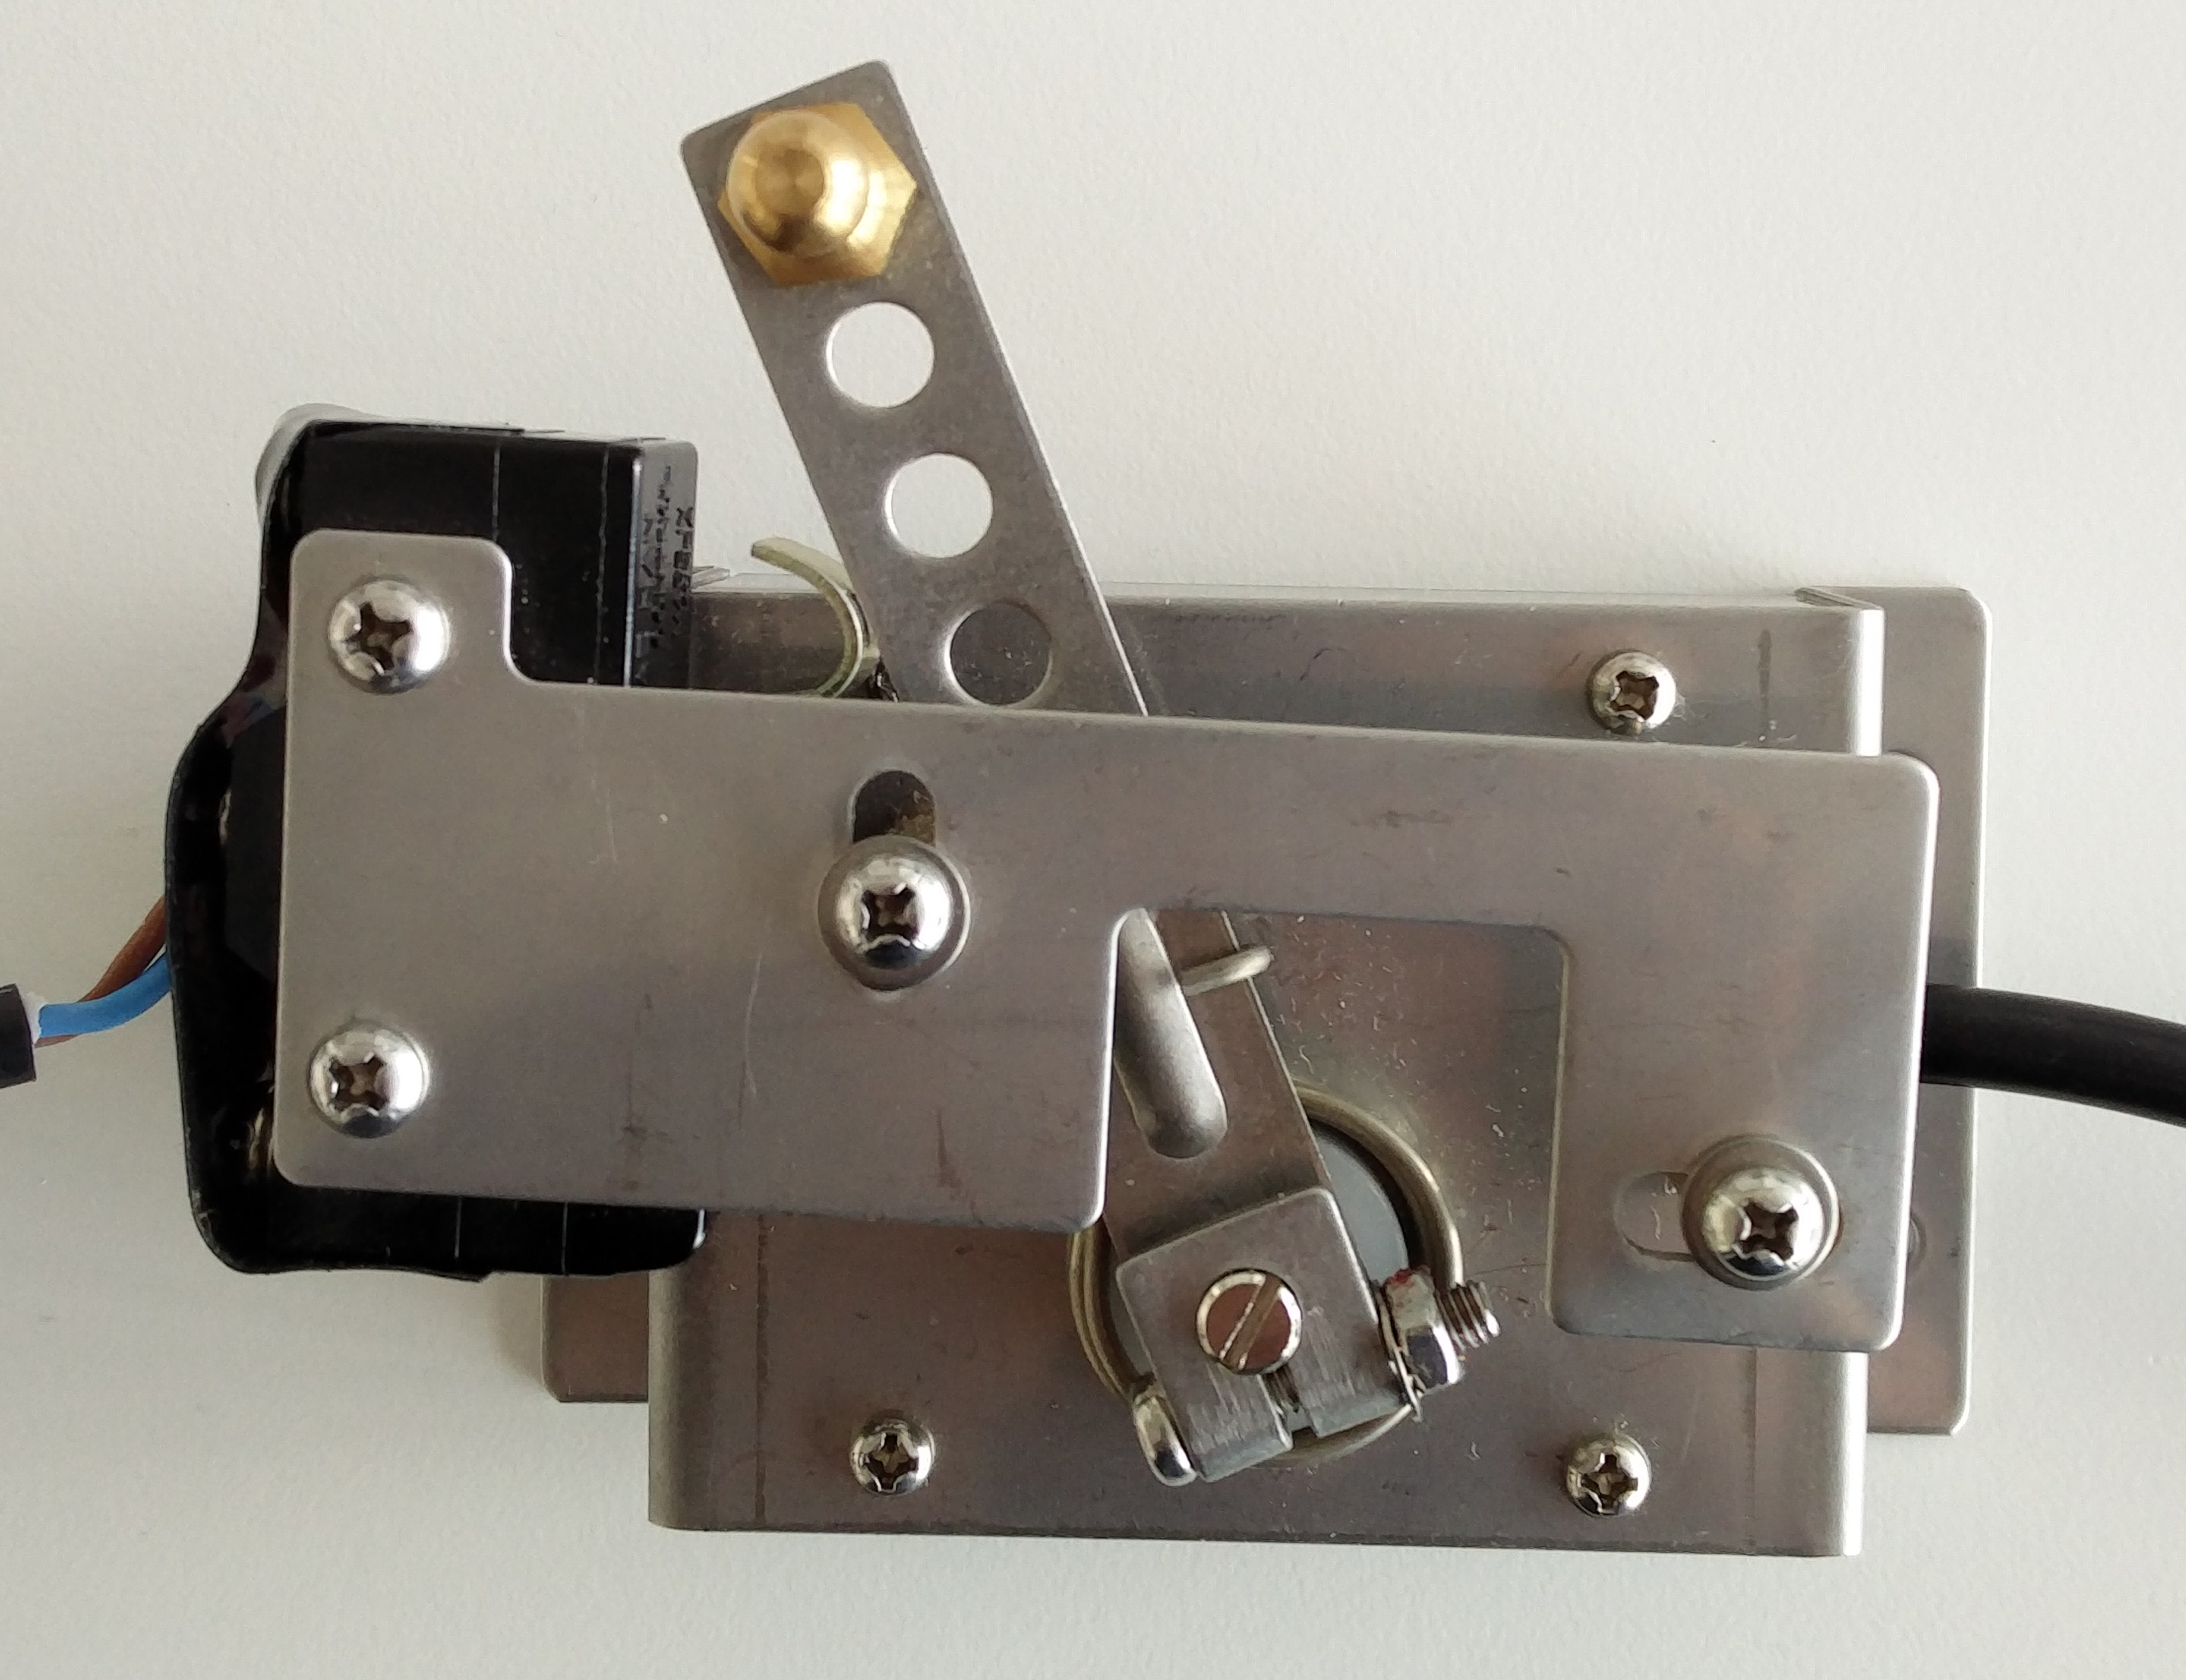
\includegraphics[width=\textwidth]{graphics/torque_pedal_picture}
		\caption{Picture of the actual torque pedal}
		\label{fig:Torque_pedal_picture}
	\end{subfigure}
	\caption{Diagram and picture of the torque pedal}
	\label{fig:Torque_pedal_diagram}
\end{figure}

\subsection{Switches and Wiring}
The wiring of the kart frame is not pre-assembled, but has been provided by the supervisors of the project, as this is standardized across multiple projects. 
A diagram of the wiring can be seen on figure \ref{fig:Kart_wiring_diagram}.\newline

The diagram shows the Sevcon Gen4 controller as the centrepiece surrounded by the other active parts. 
The motor to the right. 
The torque pedal, battery, undervoltage protection and multiple switches to the left. 
The switches include a key switch to turn the system on, an emergency switch, and a drive enable switch with three positions to change between driving forwards, reversing or disabling drive at the neutral position.

\begin{figure}[!h]
	\centering
	\includegraphics[width=.95\linewidth]{graphics/Electrical_wiring_diagram_ver3}
	\caption{Go-Kart wiring diagram}
	\label{fig:Kart_wiring_diagram}
\end{figure}

\clearpage
\section{System Overview}
To get an overview of the system connections and all the major components needed to make the kart run, a system diagram is made. Figure \ref{fig:blockdiagram1} shows the general wiring of the system. \newline

The highlighted green component is the zynq board controller. To the right of the control board is the PMAC motor and the driver and inverter to power it. The two blocks nexto the motor are the LEM current sensors. Two of these is enough because the third current can be calculated by using KCL.
Beyond the motor is the encoder producing motor positional data for the control. We might not need all three of the encoder signals but they will be routed to the control board anyway just in case. \newline

On the left side of the Zynq board is the different precautions and emergency switches at the top. These will ensure that starting, stopping and emergency procedures are completed safely without any capaictors or MOSFETS burning.
Below these switches is the undervoltage protection circuit which ensures that the kart is only driving when sufficient power is supplied. The final parts to the left are the torque pedal or speeder for the kart, and the battery supply.


\begin{figure}[!h]
	\centering
	\includegraphics[width=.85\linewidth]{graphics/wiringdiagram}
	\caption{Wiring diagram with zybo}
	\label{fig:blockdiagram1}
\end{figure}




\begin{figure}[!h]
	\centering
	\includegraphics[width=.85\linewidth]{graphics/block_diagram}
	\caption{Block diagram}
	\label{fig:blockdiagram2}
\end{figure}
%\section{Supply}
Battery info

%\subsection{Requirements}
%\subsection{Analysis}
%\subsection{Conclusion}
%\section{Current Transducer - LF 205-S}
The LF 205-S utilises the Hall effect in order to measure the current flowing through a wire.
Figure \ref{fig:lf205function} depicts an equivalent circuit of the functionality of the transducer.
As can be seen, the LF 205-S functions like a transformer.
As per the datasheet this transformer has a 1:2000 turns ratio, therefore the secondary current, $I_S$ can be found as:
\begin{equation}
	\frac{I_S}{I_P}=\frac{N_P}{N_S} \quad \Rightarrow \quad I_S = \frac{I_P}{N_S}
\end{equation}
Essentially, the LF 205-S generates a current proportional to the current flowing through the device, the primary current; $I_P$.
By changing the value of the resistor $R_m$, the resulting voltage drop can be dictated.

In section \todo[inline]{Thomas: Section documenting the maximum current to be expected in each phase.} the maximum current to be expected in each phase is found to be 300$A$.
As described in section \todo[inline]{Thomas: section on the zybo adc}, the ADC on the Zynq chip can work on signals in the ranges 0$V$-1$V$ or $\pm0.5V$.
Since the current is sinusoidal it can be negative.
Choosing the range $\pm0.5V$ therefore simplifies the circuitry needed to read the value correctly.
Consequently $R_m$ needs to be set such that the maximum expected current results in the maximum allowed voltage.
However, it is desirable to leave some headroom in case of an overcurrent event, 50$mV$ should be sufficient.
Thus:
\begin{equation}
	R_m = \frac{0.45}{I_{Pmax}/N_S} = 3\Omega
\end{equation}
  
%!TEX root = ../main.tex

\section{Electronics Design}
\label{sec:electronics}
\todo[inline]{We should have a very broad introduction somewhere. With diagrams of all the electric board. We should write somewhere that we chose the 3-phase driver and why.  - Mikkel.}

This section is dedicated to describing the electronics designed throughout this report.
This includes an analog, a digital and a power board, as well as a driver board.
Each of these boards, the choice of components and the layout will be discussed in appropriate detail in the following sections.
One aspect of the layout specifically is important; the grounding layout.
As this discussion provides a convenient means of giving an overview of the various components, the grounding will be discussed initially:

\subsection{Electronics Components and Ground Layout}
\todo{Thomas: Someone needs to verify/elaborate on my claims about noise below}
As previously mentioned, there are four boards in this design.
Across these four boards are three different ground planes: digital ground (GNDD), analog ground (GNDA) and power ground (GNDP).
Keeping these seperate is done mainly to avoid noise propagating throughout the circuits.
For instance, GNDP is used as the return path of the high currents flowing through the motor.
The voltage on this rail is likely to be fluctuating significantly.
This will surely compromise the integrity of more crucial signals such as the current measurements used to determine the position of the rotor.
GNDD will also carry significant noise from the digital circuitry and should also be kept separate from GNDA.
The only crossover between the GNDD and GNDA will happen in the DRV8301DCA (see section \ref{sec:driverboard}) and in the NOR circuitry described in section \ref{sec:nor}.
The latter occurs at the over-current event signal which is generated on the analog board but used in the digital system.
An analog signal is fed to the SN74LVC1G17, a buffer with built-in Schmitt-trigger circuitry which is supplied from the digital 3.3$V$ rail.\\
A simplified overview of the grounding planes can be seen on figure \ref{fig:groundplanes}.

\begin{figure}[!h]
	\centering
	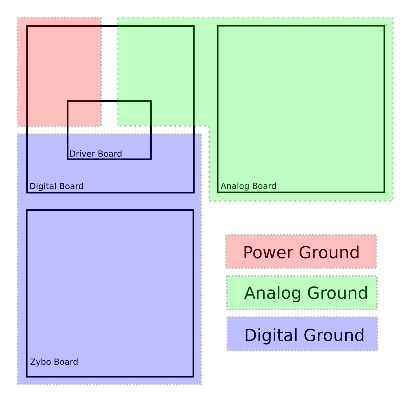
\includegraphics{graphics/ground_plane}
	\caption{Simplified view of the electronics with the ground planes marked.}
	\label{fig:groundplanes}
\end{figure}

As it is undesirable to have the potentially noisy GNDP present on the boards, it is constrained to one corner of the digital board.
Here it is used to supply the TEN20-4823WIN and the TVN5-4811WI isolated dc-dc converters that generate the $\pm15V$ and $5V$ rails respectively.
The previously mentioned 3.3$V$ rail is generated on the Zybo board.
The driver chip (The DRV8301DCA is discussed in more detail in section \ref{sec:driverboard}), is also supplied from the power rail, and as such GNDP is extended to a corner of the driver board.
Limiting the extent of GNDP is also the reasoning behind generating the $\pm15V$ rail on the digital board, even though it is used exclusively on the analog board.
An extended discussion of the grounding planes as well as the actual layout can be found in appendix

\subsection{Analog Board}
The analog board houses, as the name implies, all of the analog signal processing.
Mainly the over-current protection, but also the torque pedal scaling is present on this board.

\subsubsection{Over-current Protection}
In order to protect the system, it is necessary to create some form of over-current protection, OCP.
Three choices immediately present themselves:
\begin{enumerate}
	\item The DRV8301 is equipped with current sensing circuitry that allows the chip to automatically shut down the drivers when an over-current event, OCE, occurs.
	This requires the use of external shunt resistors to divert some of the current through the mosfets to the current sensors.
	\item Since the LF 205-S current transducers are used to measure the current through each of the phases, these measurements could be scaled such that they fulfil the role of the shunt resistors, still utilizing the built-in OCP of the DRV8301.
	\item Build circuitry that, based on the measurements done by the current transducers, detects an OCE and turns off the drive signals. 
\end{enumerate}
Initially 2 seemed like a sensible choice, however it was not possible to deduce the functionality of the OCP in the DRV8301 based on the datasheet.
Therefore it was decided to use 3 since the function will be well known and can be easily adjusted to meet any altered requirements, should the need arise.\\

Since only two phases are measured directly it is necessary to calculate the third.
This is done using a non-inverting summing amplifier.
See figure \ref{fig:sumamp}.
The output of this amplifier is given by:
\begin{equation}
	V_{out} = \left(1+\frac{R_4}{R_3}\right)\left(V_1\frac{R_2}{R_1+R_2}+V_2\frac{R_1}{R_2+R_1}\right)
\end{equation}

No amplification of the signals is wanted, thus the resistances are all set to $R=20k\Omega$. \todo{Thomas:Need correct values from Klaus/Martin}
With all three phase signals available it is possible to process them to detect any OCE's. 

\begin{figure}
	\centering
	\noindent\makebox[\textwidth]{\includegraphics[width=2\linewidth, trim=0cm 9cm 0cm 8cm]{graphics/sumamp}}
	\caption{The non-inverting summing amplifier used to calculate the current in the third phase.}
	\label{fig:sumamp}
\end{figure}

\begin{figure}
	\centering
	\includegraphics[width=\linewidth, trim=0cm 6cm 0cm 5cm]{graphics/ocp_phase}
	\caption{One phase of the over-current protection circuit.}
	\label{fig:ocpcircuit}
\end{figure}

The entire protection circuit for one phase can be seen in figure \ref{fig:ocpcircuit}.
Here the circuit has been split in accordance with the functionality of its four main parts: ADC isolation, full wave rectifier, thresholding circuit and an inverter.
Each part will be explained in appropriate detail in the following paragraphs.

\paragraph{ADC Isolation:}
The current measured in each phase is used in the control of the motor and as such it is important to maintain the integrity of the signal.
Therefore, after routing the signal to the ADC it is applied to the OCP circuit through a voltage follower.
Since the op amp has extremely high input resistance ($10^{12}\Omega$ in the case of the LF353 used in this circuit) what happens on the output-side of the voltage follower has no meaningful impact on the input-side.

\paragraph{Full Wave Rectifier:}
The phase signals are sinusoids with an expected peak amplitude of $\pm0.5V$.
In order to only needing to detect a positive OCE the signal is rectified.
Due to the small magnitude of the signals it is necessary to use a precision full wave rectifier.
The rectifier used here can be divided into two subcircuits; a half-wave rectifier and a summing amplifier.
In order to show the functionality of the rectifier, three test points are marked on the circuit, $V_i$, $V_r$, and $V_o$.
$V_i$ is the input voltage, $V_r$ is the rectification stage and $V_o$ is the rectified signal.
Figure \ref{fig:rectifier} shows the voltages at these points.

\begin{figure}
	\centering
	\includegraphics[width=\linewidth]{graphics/rectifier}
	\caption{The condition of the signal at points $V_i$, $V_r$ and $V_o$ in the full wave rectifier.}
	\label{fig:rectifier}
\end{figure}



\paragraph{Thresholding:}
As explained in section \ref{sec:lemsensor}, the input signal to the OCP circuit is dimensioned such that the maximum current in either of the phases will result in a voltage of 0.5$V$.
Also mentioned in this section is the desire to leave some headroom in case of an OCE.
This is due to the response time of the system.
50$mV$ is estimated to be sufficient.
An OCE is therefore defined as a time where the voltage exceeds 0.45$V$.
In order to avoid repeatedly switching the signal on and off, it was decided to use a Schmitt trigger.
Determining the component values is done using the following equations:

\begin{align}
	\frac{V_{cc}-V_h}{R_{7}}&=\frac{V_h}{R_8}+\frac{V_h-V_{ref}}{R_6} \label{eq:vhigh}\\
	\frac{V_{dd}-V_l}{R_{7}}&=\frac{V_l}{R_8}+\frac{V_l-V_{ref}}{R_6} \label{eq:vlow}
\end{align}

Where $V_{ref}=2.5V$ as set by the LM4040\footnote{Precision 2.5$V$ voltage reference}, the supply voltage $V_{cc}=15V$.
The desired hysteresis voltages $V_h$ and $V_l$ are $0.475V$ and $0.25V$ respectively.
This ensures that the enable signal will be pulled low when the current through any of the phases exceeds 285$A$, and will not return until the current is below 150$A$.
The LM4040 supplies a voltage in, effectively the same manner as a linear voltage supply.
It is therefore desirable to draw as little current from the component, that is, through $R_6$, as possible.
As per the datasheet it can operate from 60$\mu A\rightarrow15mA$.
It was decided to set the maximum current through $R_6$, $\frac{V_{ref}-V_l}{R_6} = I_{R_6}=100\mu A$.
This sets $R_6 = 22.5k\Omega$.
$R_7$ and $R_8$ can now be isolated using \ref{eq:vhigh} and \ref{eq:vlow}:

\begin{align}
	R_7 &= \frac{(V_{cc}V_l-V_{dd}V_h)(V_l-V_{ref})}{I_{R_6}(V_h-V_l)V_{ref}}\label{eq:r7}\\
	R_8 &= \frac{(V_{cc}V_l-V_{dd}V_h)(V_l-V_{ref})}{I_{R_6}(V_{cc}(V_l-V_{ref})-V_{dd}(V_h-V_{ref})+(V_h-V_l)V_{ref})}\label{eq:r8}
\end{align}

Resulting in $R_7 = 150k\Omega$ and $R_8 = 2542.37\Omega$.
Since 2542.37$\Omega$ is hardly a standard value, the nearest standard value is chosen such that $R_8=2550\Omega$.

\paragraph{Inverter:}
Due to the NOR-stage described in section \ref{sec:nor}, it is necessary to invert the signal.
A simple comparator is used to achieve this effect.
The input voltage to this stage is either $V_{cc}$ or $GNDD$, the voltage on the non-inverting terminal is therefore not critical.
Setting $R_9=R_{10}=10k\Omega$ is sufficient.

The circuitry discussed above will ensure that in case of an OCE, a signal is sent to the digital board where it will be used to safely handle the event.
This is discussed in further detail in later sections. 

\subsubsection{Current Transducer - LF 205-S}
\label{sec:lemsensor}
While these current sensors are not strictly part of the analog board, the circuitry related to them is and therefore it was chosen to include their description here.
The LF 205-S utilises the Hall effect in order to measure the current flowing through a wire.
Figure \ref{fig:lf205function} depicts an equivalent circuit of the functionality of the transducer.
As can be seen, the LF 205-S functions like a transformer.
As per the datasheet this transformer has a 1:2000 turns ratio, therefore the secondary current, $I_S$ can be found as:
\begin{equation}
	\frac{I_S}{I_P}=\frac{N_P}{N_S} \quad \Rightarrow \quad I_S = \frac{I_P}{N_S}
\end{equation}
Essentially, the LF 205-S generates a current proportional to the current flowing through the device, the primary current; $I_P$.
By changing the value of the resistor $R_m$, the resulting voltage drop can be dictated.

In section \todo[inline]{Thomas: Section documenting the maximum current to be expected in each phase.} the maximum current to be expected in each phase is found to be 300$A$.
As described in section \todo[inline]{Thomas: section on the zybo adc}, the ADC on the Zynq chip can work on signals in the ranges 0$V$-1$V$ or $\pm0.5V$.
Since the current is sinusoidal it can be negative.
Choosing the range $\pm0.5V$ therefore simplifies the circuitry needed to read the value correctly.
Consequently $R_m$ needs to be set such that the maximum expected current results in the maximum allowed voltage.
However, it is desirable to leave some headroom in case of an OCE, 50$mV$ should be sufficient.
Thus:
\begin{equation}
	R_m = \frac{0.45}{I_{Pmax}/N_S} = 3\Omega
\end{equation}

\subsubsection{Torque Pedal Downscale}
The torque pedal is simply a variable resistor, $R_{tp}=7.5k\Omega$. \todo[inline]{Thomas: Verify resistor value on final system}
As the pedal is actuated the resistance changes.
Figure \ref{fig:torquepedaldownscale} is a depiction of the circuit used to read the position of the torque pedal.
$R_1$ and $\mathrm{R_P}$ form a variable voltage divider of the $15V$ rail.
The analog input of the ADC in the FPGA, however, is limited to 0-1$V$.
Therefore it is necessary to downscale the voltage.
Intuitively this could be done using simply a voltage divider, but since the torque pedal functions as a voltage divider, the varying resistance distribution of the torque pedal would influence the voltage divider.
For this reason a voltage follower is used to isolate the two circuits.
In addition, a 5.1$V$ zener diode is clamping the signal to ground in order to protect the ADC of the FPGA.
\todo{capacitor for noise}
\begin{figure}[!h]
	\centering
	\includegraphics[width=.75\linewidth]{graphics/torque_pedal_downscale}
	\caption{Circuit used to scale the voltage from the torque pedal from $0V\rightarrow5V$ to $0V\rightarrow1V$.}
	\label{fig:torquepedaldownscale}
\end{figure}

The resistance of the pedal changes linearly, which means the voltage division does not. Voltage at the point TP as a function of pedal is:

\begin{equation}
V_{TP}(R_P) = V_{CC} \frac{R_P}{R1 + PEDAL} \frac{R3}{R3 + R2}
\label{eq:pedal_voltage}
\end{equation}

By isolating $\mathrm{R_P}$, it's possible to calculate what its resistance is. 
The resistance of $\mathrm{R_P}$ varies from $0$ to $7.5 k\Omega$, as the pedal is pressed down. 
Hence, equation~\ref{eq:pedal_back_calc} will give a value proportional to the torque requested by the driver

\begin{equation}
R_P = \frac{V_{TP} R1 \cdot (R2 + R3)}{R3 \cdot (V_{CC} - T_{TP}) -  V_{TP} \cdot R2}
\label{eq:pedal_back_calc}
\end{equation}

Finally, due to the mechanical nature of the torque pedal, this signal is likely to be noisy.
C$_1$ is placed in order to filter this noise.

\begin{figure}[H]
	\begin{center}
		\includegraphics[width=10cm]{graphics/pedal_voltage.pdf}
		\label{fig:pedal_voltage}
		\caption{Voltage as a function of the pedal resistance.}
	\end{center}
\end{figure}

\subsection{Digital Board}
The digital board is used mostly as an interconnection board between the various electronic components in the system.
The logic levels of the different systems are managed here along with the enable signal for the DRV8301.

\subsubsection{Drive Enable Signal}
This signal is produced by the torque pedal.
When the user actuates the pedal a switch is connected to ground. 
By reading the drive enable signal it is therefore possible to determine when the controller should be running, allowing a means for avoiding integral windup.
Since this signal is left floating when the pedal is not active, it can be routed directly to the Zybo, using the internal pull-up resistors.
\todo[inline]{Thomas: Is the torque pedal active low or active high? Correct two places above to reflect the correct case}
\subsubsection{Driver Enable Circuit}
\label{sec:nor}
The DRV8301DCA is equipped with a pin called \texttt{EN\_GATE}.
If, while running, this pin is pulled low, the drive signals are immediately shut down.
This feature allows for fast and reliable shut down of the motor in case of any detected faults.
There are two different types of faults detected within the system, the aforementioned OCE and an over-temperature event, OTE.
In addition to these two a signal is routed from the Zybo which enables the digital part of the system to disable/enable the motor, should the need arise.
As there are three different signals that all need to connect to the same pin, they are all NOR'ed, as seen in figure \ref{fig:driveenablesignal}.

\begin{figure}[!h]
	\centering
	\includegraphics[width=\linewidth,trim=0cm 3cm 0cm 3cm]{graphics/driver_enable_signal}
	\caption{The NOR circuit that compares the three enable signals to determine whether the drive signals should be on.}
	\label{fig:driveenablesignal}
\end{figure}

The observant reader will notice that two 2-input NOR gates was used rather than one 3-input gate.
Reason for this is that the OTE protection was not implemented until after the components were ordered.
In order then to not need additional components it was decided to cascade the available component.
This cascading however does mean that it is necessary to invert the logic level of the signals OCE, and OTE.
OCE is inverted on the analog board while OTE is used to pull the signal to ground.
The two signals are both routed to the Zybo.
This is done such that it is possible to discern which event has triggered when the motor halts.

\subsubsection{Logic-Level Shifters}
Tracking the angular position of the rotor is done using an encoder mounted on the motor.
Upon receiving a clock signal the encoder will return the current position of the rotor.
The encoder module is an AM256 which, according to the datasheet, requires at least 3.5$V$ for digital high input.
However, the Zybo uses 3.3$V$ and the clock signal therefore needs to be shifted to the correct voltage level, 5$V$. 
A, B, Z and Data generated by the AM256 all need to be shifted down to 3.3$V$ in order to protect the Zybo.
The circuit for these four signals can be seen in figure \ref{fig:lls}.
The buffer used for these signals is, as can be seen from the figure, the 74AHC125 which is a quad-buffer.
$V_{out}$ of this device is equal to $V_{cc}$, while $V_{in}$ can be any voltage from $0\rightarrow 5V$, by supplying it from the 3.3$V$ rail it will therefore act as a logic level shifter.

\begin{figure}[!h]
	\centering
	\includegraphics[width=.5\linewidth,trim=0cm 1cm 0cm 1cm]{graphics/lls}
	\caption[Logic level shifter circuit.]{The 74AHC125 quad-buffer used to shift the logic level of the encoder from 5$V$ down to the $3.3V$ required by the Zybo. Due to an oversight, a buffer with an enable on each port was bought. This feature is unnecessary and they are always enabled.}
	\label{fig:lls}
\end{figure}

\subsection{Driver Board}
This is not finished!
\label{sec:driverboard}

\subsubsection{SPI}
The DRV8301 is capable of performing SPI communication as a slave.
This can be used to read status registers of the chip and set configuration options.
%!TEX root = ../main.tex
\section{Embedded Design}\label{sec:Embedded_Design}
\label{sec:emb}
An embedded system is needed to handle a wide range of task. 
It is a requirement for the project that the Zybo board should be used as the embedded system in the project.
The Zybo board features a Zynq Z-7010 chip from Xilinx, which has an integrated dual-core ARM Cortex-A9 processor and a Xilinx 7-series field programmable gate array (FPGA).
The Zybo board itself consists, among other, of several buttons, switches, LEDs and connections for USB, Ethernet, HDMI and several PMOD connectors. 
Throughout the remainder of the report the FPGA part will be referred to as the Programmable Logic (PL) and the ARM processor as the Processing System (PS). 


\subsection{Functionality}
An analysis of the complete system yielded the functionalities listed below for the Zybo board. 

\begin{itemize}
\item Digital inputs and outputs
\item Generating PWM
\item Measuring voltage output from LEM sensors and torque pedal
\item UART communication with external PC
\item Control algorithms for dq-control
\item Read position from encoder
\item SPI communication as master
\end{itemize}

As can be seen on the list there are multiple tasks that needs to be handled. 
Optimally, these tasks should be run at different speeds.
For instance, the PWM switching frequency should be 20\si{\kilo\hertz} as described in section \ref{sec:inverter}.
As this is quite fast it should be handled in PL. 
The rest can be handled in PS.
In order to more easily run tasks at different frequencies it was chosen to use khaOS, a Run To Complete Scheduler (RTCS) system made by Karsten Holm Andersen.
Using an RTCS simplifies scheduling tasks to run at different frequencies.

As an RTCS has no way to preempt tasks it leaves the responsibility of preserving real time performance of the system to the programmer.
khaOS was chosen before other RTCS as the group had prior knowledge about the system from an Embedded Systems course.

\subsection{Architecture}
The software functionalities are grouped into tasks based on functionality and desired frequency.
A task diagram of the complete system on the Zybo can be seen in figure \ref{fig:task_diagram}.

%\begin{figure}[!h]
%	\includestandalone[width=\textwidth]{graphics/taskdiagram}
%	\caption[Task diagram]{Task diagram showing software tasks as green circles, shared variables as yellow boxes, IP cores as blue boxes, I/O periphirals as limegreen oxes, % external signals as orange boxes and external components in red. The PS and PL areas are marked accordingly and arrows show the data and signal direction.}
%	\label{fig:task_diagram }
%\end{figure}

\begin{figure}[!h]
  \includegraphics[width=\textwidth]{graphics/taskdiagram}
  \caption[Task diagram]{Task diagram showing software tasks as green circles, shared variables as yellow boxes, IP cores as blue boxes, I/O peripherals as lime green boxes, external signals as orange boxes and external components as red boxes. The PS and PL areas are marked accordingly and arrows show the data and signal direction. $C_p$ consists of various controller parameters.}
  \label{fig:task_diagram}
\end{figure}

As can be seen, various signals are coming from the outside world through the PL into the PS.
All tasks, IP cores and I/O peripherals will be described in the coming sections.

\subsubsection{Three phase PWM generator}
The PWM generator is placed in the PL and is developed using Xilinx System Generator in Matlab Simulink.
The generator is made to have adjustable frequency and duty cycle.
It was chosen to generate center aligned PWM as this introduces less harmonic distortion than edge aligned PWM \cite{power_switching_converters}. 
Furthermore center aligned PWM has the benefit of producing symmetrical PWM.
Symmetrical PWM has a well defined midpoint where the current can be sampled correctly. \todo[inline]{Thomas: Do you ever touch on why it is difficult to sample correctly?}
The high limit for the counter can be calculated for a given frequency, $f$, by the following:
$$H = L + \frac{f_{Zybo}}{f\cdot 2}$$
Where H is the high limit, L is the low limit and $f_{zybo}$ is the Zybo clock frequency.
The PWM counter system can be seen in figure \ref{fig:pwm_counter}.
The counter block will count up or down depending on the input. 
The output from the counter value will go into to two compare blocks along with the high and low limits.
The compare blocks will produce a high signal when the counter value is equal either the high or low limit.
These signals are then fed to an m-code block which contains a simple state machine which determines the direction of the counter.
\begin{figure}[!h]
	\centering
	\includegraphics[width=0.8\linewidth]{graphics/counter}
	\caption[Block diagram of counter in PWM generator.]{Simulink block diagram of the counter in the PWM generator.}
	\label{fig:pwm_counter}
\end{figure}
The counter out signal can be seen in figure \ref{fig:pwm_graph}.
This signal is then fed into the PWM generator shown in figure \ref{fig:pwm}. 
The duty cycle is given to the PWM generator as data type u32, an integer type.
Therefore the dutycycle is given in a range of 0 to 1000, giving a resolution of 0.1\%.
The switching limit is the value, where when the counter value equals, switches the polarity of the PWM output.
The switching limit is calculated from the following:
$$l = (1 - \frac{d}{1000}) \cdot r$$
Where l is the switching limit, d is the dutycycle in the range 0 - 1000 and r is the counter range.
A register will then make sure that the switching limit is only applied when the counter is lowest.
This is important as otherwise the dutycycle may be corrupted by misaligning the PWM.
The compare block will make the PWM signal by comparing the switcing limit to the counter value.
The counter signal and output of the PWM generator can be seen in figure \ref{fig:pwm_graph}.
As the PWM generator should be able to do three independent PWM signal there are three of the systems shown in figure \ref{fig:pwm}, one for each phase.

\begin{figure}[!h]
	\centering
	\includegraphics[width=1\linewidth]{graphics/pwm_system}
	\caption[Block diagram of PWM generator.]{Simulink block diagram of the PWM mechanism in the PWM generator.}
	\label{fig:pwm}
\end{figure}

\begin{figure}[!h]
	\begin{center}
		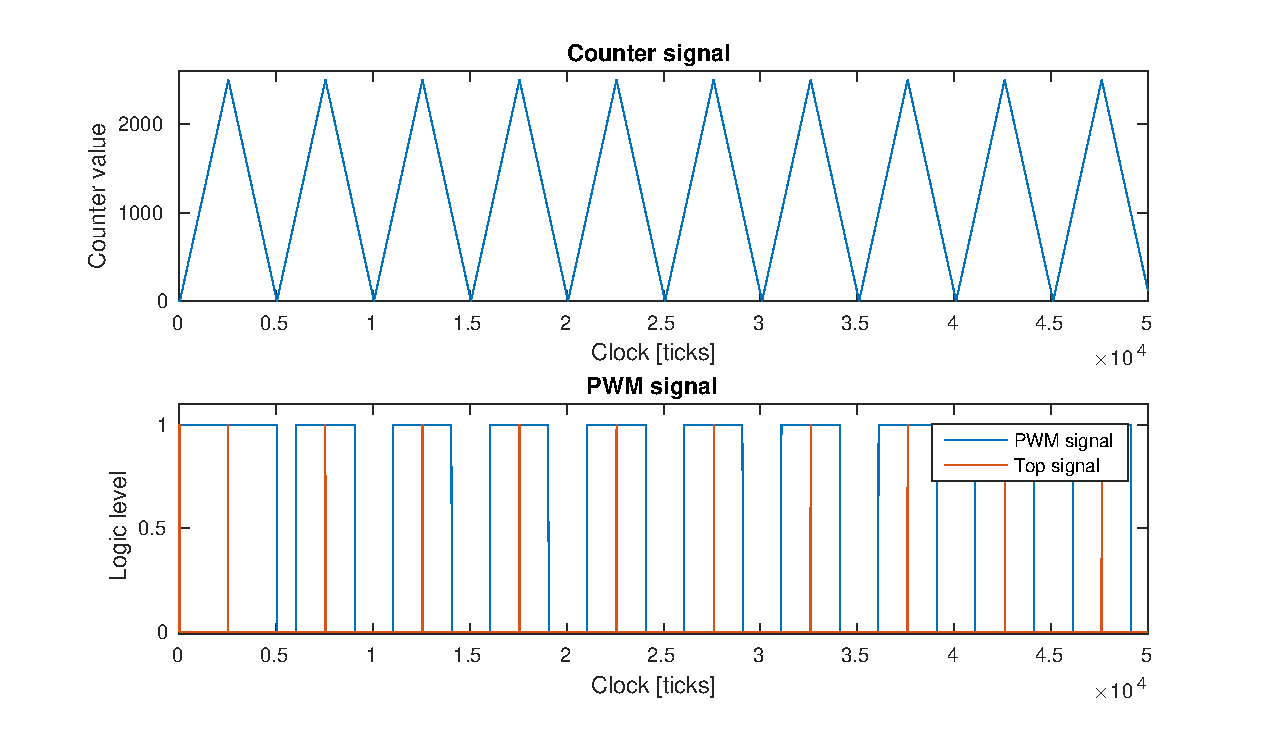
\includegraphics[width=\linewidth]{graphics/pwm_plot}
		\caption{Counter and PWM signal.}
		\label{fig:pwm_graph}
	\end{center}
\end{figure}


\subsubsection{Interface task}
The interface task reads external signals, outputs digital signals and controls the other tasks.
This includes ensuring that the state of the enable variable, read by the controller and the PWM task, is correct.
The basic functionality of the interface task can be seen in the flowchart of figure \ref{fig:interface}.

%\begin{figure}[!h]
%	\centering
%	\includegraphics[width=0.7\linewidth]{graphics/interface_task}
%	\caption[Block diagram of PWM generator.]{Simulink block diagram of the counter in the PWM generator.}
%	\label{fig:interface}
%\end{figure}

\begin{figure}[!h]
	\centering
	\includestandalone[width=0.5\textwidth]{graphics/interface_flow}
	\caption[Interface task.]{Flow chart illustrating the basic functionality of the interface task.}
	\label{fig:interface}
\end{figure}

At startup the interface task switches on the inrush relay for a certain time.
Afterwards the main relay is switched on and the inrush relay is switched off after some time to ensure that the main relay is conducting.
Then the task will read all signals from the digital board and, if \texttt{EN\_GATE} is high, the global enable variable will be set high.
If \texttt{EN\_GATE} is low, indicating a fault, the task will change the enable variable to low.
Alongside the functionality shown in figure \ref{fig:interface}, the interface will act as master for the two UART tasks.
This enables the setting of values within the system as well as potentially reading the current status of the system.
All communication through the UART interface is done through the \texttt{rx\_buffer} and \texttt{tx\_buffer} arrays shown in listing \ref{lis:uartvars}.
Currently three parameters can be set within the system:
\begin{itemize}
	\item \texttt{kp/ki}: These are the values of the PI controller used.
	\item \texttt{qmax}: The limit of the current that the controller is allowed to set as reference. 
\end{itemize}
Setting any of the above is done by:
\begin{center}
\texttt{set <parameter> <value>}
\end{center}
As can be seen in listing \ref{lis:cutcommand} the command is split into parts using \texttt{strtok()}.
This is a non-reentrant function that will return all the characters until the first appearance of delimiter.
Every consecutive call to the function with \texttt{NULL} as the first parameter will continue the search through the same array.
With the command split into tokens it is parsed using a simple if-structure, comparing each argument in the command using \texttt{strcmp()} until a value can be set.

\begin{lstlisting}[captionpos=b,style=customCpp, caption={Something clever!.THOMASSSS!}, label=lis:cutcommand, escapeinside={(*@}{@*)}]
if(rx_flag)
{
  char* cmd = strtok(rx_buffer, DELIMITER);
  char* var = strtok(NULL, DELIMITER);
  char* val = strtok(NULL, DELIMITER);
  
  if(!strcmp(cmd,"set"))
  {
    if(!strcmp(var,"kp"))
    {
      scanf(val, "%f", &kp);
      sprintf(tx_buffer, "kp was set: %f", kp);
      tx_flag = true;
      tx_tail = strlen(tx_buffer);
    }
  	
(*@\makebox[.25\linewidth][c]{$\smash{\vdots}$}@*)
  
  }
  rx_flag = false;
  rx_tail = 0x00;
}
\end{lstlisting}

Once the value is set a message is returned to the user, informing of the successful setting.
\texttt{rx\_flag} is cleared and the buffer is emptied by setting \texttt{rx\_tail} to zero.
The system is made with expandability in mind, currently only a \texttt{set} command is implemented.
This could easily be extended to a \texttt{read} or perhaps a \texttt{shutdown} command.

\subsubsection{Controller task}
\begin{figure}[!h]
	\centering
	\includestandalone[width=0.9\textwidth]{graphics/tikz/Block_diagram1tikz}
%		\includegr%aphics[width=0.9\linewidth,trim=3cm 15cm 0 2cm]{graphics/controller_tasktikz}
	\caption[Block diagram of controller task.]{Block diagram showing the functionality of the controller task.}
	\label{fig:controller_task}
\end{figure}

The basic functionality of the controller task can be seen in figure \ref{fig:controller_task}.
The task polls data from the ADC in order to get the raw data for the phase currents $I_a$, $I_b$ and the torque pedal.
The raw data from the ADC is then calculated into voltages and the two currents are calculated by:

\begin{equation}
	 I = \frac{V_{measured}}{R_m} \cdot NS
\end{equation}

$I_c$ is calculated based on the assumption that the three currents form a balanced three phase system.
The resistance of the torque pedal potentiometer is calculated from the measured voltage and equation \ref{eq:pedal_back_calc}.

$I_a$, $I_b$, $I_c$ and $\theta$ are then used to perform a Clarke Park transformation and obtaining the values of $I_d$ and $I_q$. 
$I_d$ and $I_q$ should be controlled towards a set point by two separate controllers.
The point for $I_d$ is 0 as will be explained in section  \ref{sec:controller_design}. 
The point, $q_{set}$, for $I_q$ should be related to the maximum allowed current, $q_{max}$, and the position of the torque pedal in percent, $pedal_\%$:
\begin{equation}
	q_{set} = pedal_\% \cdot q_{max}
\end{equation}
It was chosen to use two PI controllers as will be described in section \ref{sec:controller_design}.
The code for one of the controllers can be seen in listing \ref{lis:controller_code}.
As can been seen in line 2 trapezoidal integration is used to perform the integration. 
Lines 4-8 performs anti-windup and lines 9-14 calculates the output if enable is high and performs integrator reset if low.

\begin{lstlisting}[captionpos=b,style=customCpp, caption={[C code constituting a PI controller.]C code constituting a PI controller with trapezoidal integration, anti windup and integrator reset.}, label=lis:controller_code]
d_error = d_set - I_d_measured;
d_integral = d_integral + (d_previous_error + d_error)*0.5*dt;

if(d_integral > MAX_TOTAL_OUTPUT){
	d_integral = MAX_TOTAL_OUTPUT;
}else if (d_integral < -MAX_TOTAL_OUTPUT){
	d_integral = -MAX_TOTAL_OUTPUT;
}
if(enable){
	d_output = kp * d_error + ki * d_integral;
}else{
	d_output = 0;
	d_integral = 0;
}
d_previous_error = d_error;

\end{lstlisting}
Afterwards \texttt{d\_output} and \texttt{q\_output} are 
Afterwards the output values are downscaled if they exceed the maximum limits.
The code for downscaling can be seen in \ref{lis:saturation}.

\begin{lstlisting}[captionpos=b,style=customCpp, caption={[C code for downscaling.]C code for detecting and downscaling output values that exceed the maximum limits.}, label=lis:saturation]
total_output_magnitude = sqrt(d_output*d_output + q_output*q_output);

if(total_output_magnitude > MAX_TOTAL_OUTPUT){
	d_output = (d_output* MAX_TOTAL_OUTPUT)/total_output_magnitude;
	q_output = (q_output* MAX_TOTAL_OUTPUT)/total_output_magnitude;
}
\end{lstlisting}

\subsubsection{PWM task}
The basic functionality of the PWM task can be seen in the block diagram of figure \ref{fig:pwm_task}.
The task needs to take the outputs from the controller task and transform it into duty cycles that can be feed to the PWM generator in the PL area of the Zybo. 
The PWM task is separate from the controller task as it might be preferable to have the two tasks run at different frequencies.
The task reads the rotor position from the encoder and access the global variables \texttt{d\_output} and \texttt{q\_output}. 
This information is used to perform inverse Clarke Park transformation.
Afterwards third harmonic injection is performed and if the values are higher or lower than the maximum bounds they are limited.
The global enable variable is checked and passed to the enable pin.


\begin{figure}[!h]
	\centering
%	\includegraphics[width=0.9\linewidth,trim=2cm 17cm 0cm 4cm]{graphics/pwm_tasktikz}
  	\includegraphics[width=\textwidth]{graphics/PwmTask2}
	\caption[Block diagram of PWM task.]{Block diagram showing the functionality of the PWM task.}
	\label{fig:pwm_task}
\end{figure}

\subsubsection{ADC}
The Zynq chip contains a dual 12-bit, 1 Mega sample per second (MSPS) Analog-to-Digital Converter (ADC) \cite{adc}.
The ADC is utilized through the XADC Wizard in Vivado. 
The ADC measures the difference between differential analog input pins $V_p$ and $V_n$.
The IP core is configured to use AXI4LITE connection, simultaneous selection, unipolar mode and event mode.
Simultaneous selection mode is used as it allows simultaneous sampling on the dual ADC. 
When using simultaneous sampling the phase relationship is preserved.
When unipolar mode is enabled the input range between $V_p$ and $V_n$ is 1 \si{\volt} and the input voltage must always be positive with respect to ground.
Setting the ADC in event mode, means that the ADC will only sample when there is a rising edge on its CONVST pin. 
The CONVST pin is connected to the top signal of the PWM generator meaning that the ADC will sample in the center of the PWM pulse.
This is done to sample the current correctly. 
Channels 6 and 14 are paired together in simultaneous mode, meaning that they will be sampled simultaneously.
These are the channels that the outputs from the two LEM sensors are connected to. 
The torque pedal signal will be routed to channel 7 which will be sampled after channel 6 and 14.
The top signal from the PWM generator will start the sampling and therefore it will also set the sampling frequency.
As the PWM frequency is 20 \si{\kilo\hertz} the ADC sampling frequency will be as well.

\subsubsection{UART RX/TX}
In order to facilitate communication between the Zybo board and a PC, a small UART connection is established.
The connection consists of two tasks, UART\_RX and UART\_TX.
They handle receiving and transmitting, respectively.
As shown in listing \ref{lis:uartvars} each of the tasks are given a buffer, a flag and a tail variable.

\begin{lstlisting}[captionpos=b,style=customCpp, caption={UART\_RX/TX buffers and variables.}, label=lis:uartvars]
char rx_buffer[0xff];
char tx_buffer[0xff];
bool rx_flag = false, tx_flag = false;
uint8_t rx_tail = 0x00, tx_tail = 0x00;
\end{lstlisting}

\begin{lstlisting}[captionpos=b,style=customCpp, caption={UART\_RX task.}, label=lis:uartrx]
void uart_rx_task()
{
  if (XUartPs_IsReceiveData(UART_BASEADDR))
  {
    rx_buffer[rx_tail] = XUartPs_ReadReg(UART_BASEADDR, XUARTPS_FIFO_OFFSET);
    rx_tail++;
  }
  if(rx_buffer[rx_tail-1] == '\r')
  {
    rx_flag = true;
  }
  _wait(MILLI_SEC(1));
}
\end{lstlisting}

Looking at listing \ref{lis:uartrx} the function of these in the UART\_RX task can be seen.
If there is data on the line it is pushed onto the \texttt{rx\_buffer} and \texttt{rx\_tail} is incremented.
This is to keep track of the number of characters that have been received.
Finally, if the last character received is a carriage return, the \texttt{rx\_flag} is set high.
This indicates to the interface task that a full command has been received and is ready for execution.
Listing \ref{lis:uarttx} shows the UART\_TX task.
Every time it is run it will check \texttt{tx\_flag}.
If \texttt{tx\_flag} is high, this indicates that data has been put into the \texttt{tx\_buffer}.
All \texttt{tx\_tail} characters in the buffer are transmitted character by character.
Hereafter \texttt{tx\_buffer} is "emptied" by setting \texttt{tx\_tail} to zero and \texttt{tx\_flag} is set low to indicate that transmission is complete.
\begin{lstlisting}[captionpos=b,style=customCpp, caption={UART\_TX task.}, label=lis:uarttx] 
void uart_tx_task()
{
  if(tx_flag)
  {
    uint8_t i;
    for(i = 0; i < tx_tail; i++)
    {
      xil_printf("%c",tx_buffer[i]);
    }
    tx_tail = 0x00;
    tx_flag = false;
  }
  _wait(MILLI_SEC(250));
}
\end{lstlisting}

\subsection{Encoder}
The Zybo board needs to interface the RMB28MD encoder that is mounted on the motor.
The RMB28MD is an absolute encoder with sine/cosine, SSI and incremental output. 
It was chosen to use the SSI output as an IP core capable of reading the position by SSI communication was made available by the supervisors of the group.
Reading the position through SSI yields a resolution of 8 bit per mechanical revolution. 
The physical RMB28MD encoder signals are interfaced by an IP Core.
The IP core outputs a clock to the RMB28MD chip and reads data from a data pin. 
It then makes the data available on the AXI4LITE bus, where it can be read from software by the PWM task. 

\subsection{SPI communication}

%\begin{figure}[!h]
%	\centering
%	\includegraphics[width=1\linewidth]{graphics/spi_timing}
%	\caption[SPI timing requirements.]{SPI timing requirements.From datasheet? How to cite?}
%	\label{fig:spi_timing}
%\end{figure}

As described earlier the Zybo board will need to set certain parameters on the DRV8301 chip using SPI communication. 
The Zynq chip has two SPI controllers in the PS area of the chip, which can be setup to communicate with external devices.
By investigation of the Zynq datasheet \cite{zynq_reference} it was found that it is not possible to configure the SPI controller to meet the requirements of the DRV8301. 
More specifically, it is not possible to configure the clock signal to go low for a minimum of 40 \si{\nano\second} \cite{DRV8301}, before Slave Select goes low. 

Two solutions are proposed to solve to this problem:

\begin{enumerate}
	\item Develop a simple SPI driver in VHDL or System Generator to send the 16 bits according to the SPI requirements of the DRV8301.
	\item Use the SPI controller in PS and delay the Slave Select signal physically.
\end{enumerate}

Clearly, the correct solution to the problem is to develop an SPI driver, but due to time considarations it was decided to use the SPI controller of the Zynq.

SPI 1 on the Zynq is used as it can be ported to MIO channels 10 to 15, which can be accessed through the PMOD connectors of the Zybo board. 
The SPI controller is initialized in software and is configured to be in master mode, manual chip select mode and manual start mode by writing to the configuration register Config\_reg0.
In order to comply with the SPI specifications of the DRV8301 it was configured with the XSPIPS\_CLK\_PHASE\_1\_OPTION in order to make data valid on falling edges of the clock. 
The discharge of a capacitor is utilized to make a delay on the Slave Select signal, by putting a XX capacitor and XX resistor in series with the signal.
\todo[inline]{Thomas: Are they in series? + numbers instead of XX XX}
The transmission of \texttt{0b0001000000110000} was measured using an oscilloscope and can be seen in figure \ref{fig:spi_graph}.

\begin{figure}[!h]
	\centering
		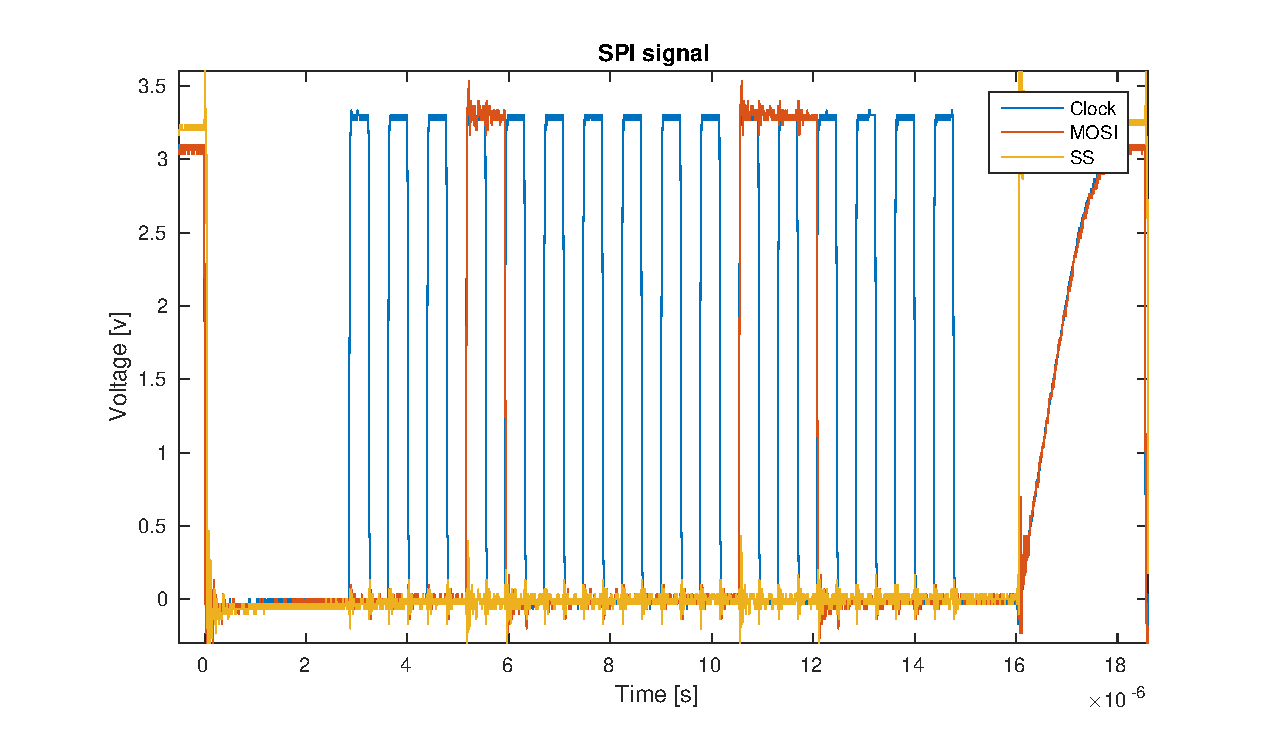
\includegraphics[width=1\linewidth]{graphics/spi}
	\caption[SPI transmission.]{SPI transmission of two data bytes.}
	\label{fig:spi_graph}
\end{figure}

\subsection{Task frequencies}
Table \ref{tabl:task_freq} shows the frequencies at which the task are run.
The PWM task will be run at 20 \si{\kilo\hertz} as this allows for updates of dutycycles at the same frequency as the PWM generator.
The controller task will run at 5 \si{\kilo\hertz} as will be explained in section \ref{sec:controller_design}.
The most essential functionality of the interface task is to update the enable variable. 
As the driver chip shuts down the inverter in case of an overcurrent event it is not very time critical to do so.
Therefore it was chosen to run the interface task at 1\si{\kilo\hertz}.
The UART tasks are not in any way crucial and can therefore be run at a low frequency, though it has to be fast enough for the user to feel that the system is responding, 100\si{\hertz} was chosen.

\begin{table}[]
\centering
\begin{tabular}{|l|l|}
\hline
\rowcolor[HTML]{C0C0C0} 
\textbf{Task} & \textbf{Frequency} 				\\ \hline
PWM     	  & 20\si{\kilo\hertz}               \\ \hline
Controller    & 5\si{\kilo\hertz}               \\ \hline
Interface     & 1\si{\kilo\hertz}              \\ \hline
UART          & 100\si{\hertz}            		\\ \hline
\end{tabular}
\caption{Table showing the frequency of each task.}
\label{tabl:task_freq}
\end{table}

\subsection{Timing}
To ensure the real time performance of the system a timing test was performed. 
An output pin was set high when entering a task and low, when exiting the task. 
PWM, controller and interface were connected to separate pins while the two UART tasks were connected to the same pin.
The voltage on the pins were measured by an oscilloscope and the measurement can be seen in figure \ref{fig:timing}.
In the first graph the tasks are in normal operation and it can be seen that the real time performance is maintained and that there is time left for expanding the tasks.
In the lower graph, the interface task is programmed to output a string to the UART transmit task, giving extra work to both tasks.
It is seen that the real time performance is still maintained even in, what is believed to be, a worst case operation.
The delay between the PWM task and the controller task can, at time of writing, not be explained.
However, it does not interfere with the functionality of the program and will, due to time constraints, not be investigated further.

\begin{figure}[!h]
	\begin{center}
		\includegraphics[width=\linewidth]{graphics/timing}
		\caption{Timing}
		\label{fig:timing}
	\end{center}
\end{figure}
\clearpage

\section{Three Phase Inverter}

%\subsection{Requirements}
%\subsection{Analysis}
%\subsection{Conclusion}
\section{PMAC Motor}\label{sec:PMAC} %by Martin

%\subsection{Requirements}
%\subsection{Analysis}
%\subsection{Conclusion}
This section focuses on the motor used for this project.
Initially the functionality of the motor will be described, then certain motor parameters will be tested, as the online product description is not all that clear.
Lastly a parking test will be performed to determine the angle of the encoder mounted on the motor. 
The motor used to drive the go-kart is an 8-pole non-salient permanent magnet synchronous motor. 

\subsection{Motor description}\label{sub:motor_descrpition}
The motor used is a 3-phase Wye-connected, 8-pole non-salient permanent magnet AC motor, the Motenergy ME1117.
Although there are many different types of PMAC motors, there is no physical difference between brushless DC motors (BLDC), permanent magnet AC motors (PMAC), and permanent magnet synchronous motors (PMSM). 
The motor will be driven as an AC or synchronous motor (since these are the same) to produce a more consistent torque.
This means that the rotor consists of four pairs of magnets - one with the north side facing outward towards the stator and one with the north side facing inward to the ferromagnetic core of the rotor. 
The stator consists of 24 solenoids mounted inward on a ferromagnetic outer ring. 
Looking at the motor from the axle side, a counter clockwise rotoration results in the go-kart going forward. See figure~\ref{fig:motor_24p}.
The solenoids are placed so that the four phase A solenoids are placed along the horizontal and vertical axes - this is not necessarily true, but a parking test will be performed in section~\ref{sub:parking_test} to determine the actual placement.
The order of the other solenoids, when going counter-clockwise is then $\bar{B}$, $C$, $\bar{A}$, $B$ and $\bar{C}$, as shown on figure~\ref{fig:motor_24p}. 
The solenoids $A$ correspond to terminal M1, solenoids $B$ correspond to M2, and solenoids $C$ correspond to M3. 
Current going into terminal M1, will then pass through all the $A$ and $\bar{A}$ solenoids in series, before reaching the star point, and continuing through $B$ and $\bar{B}$ and/or $C$ and $\bar{C}$.

\begin{figure}[H]
	\begin{center}
		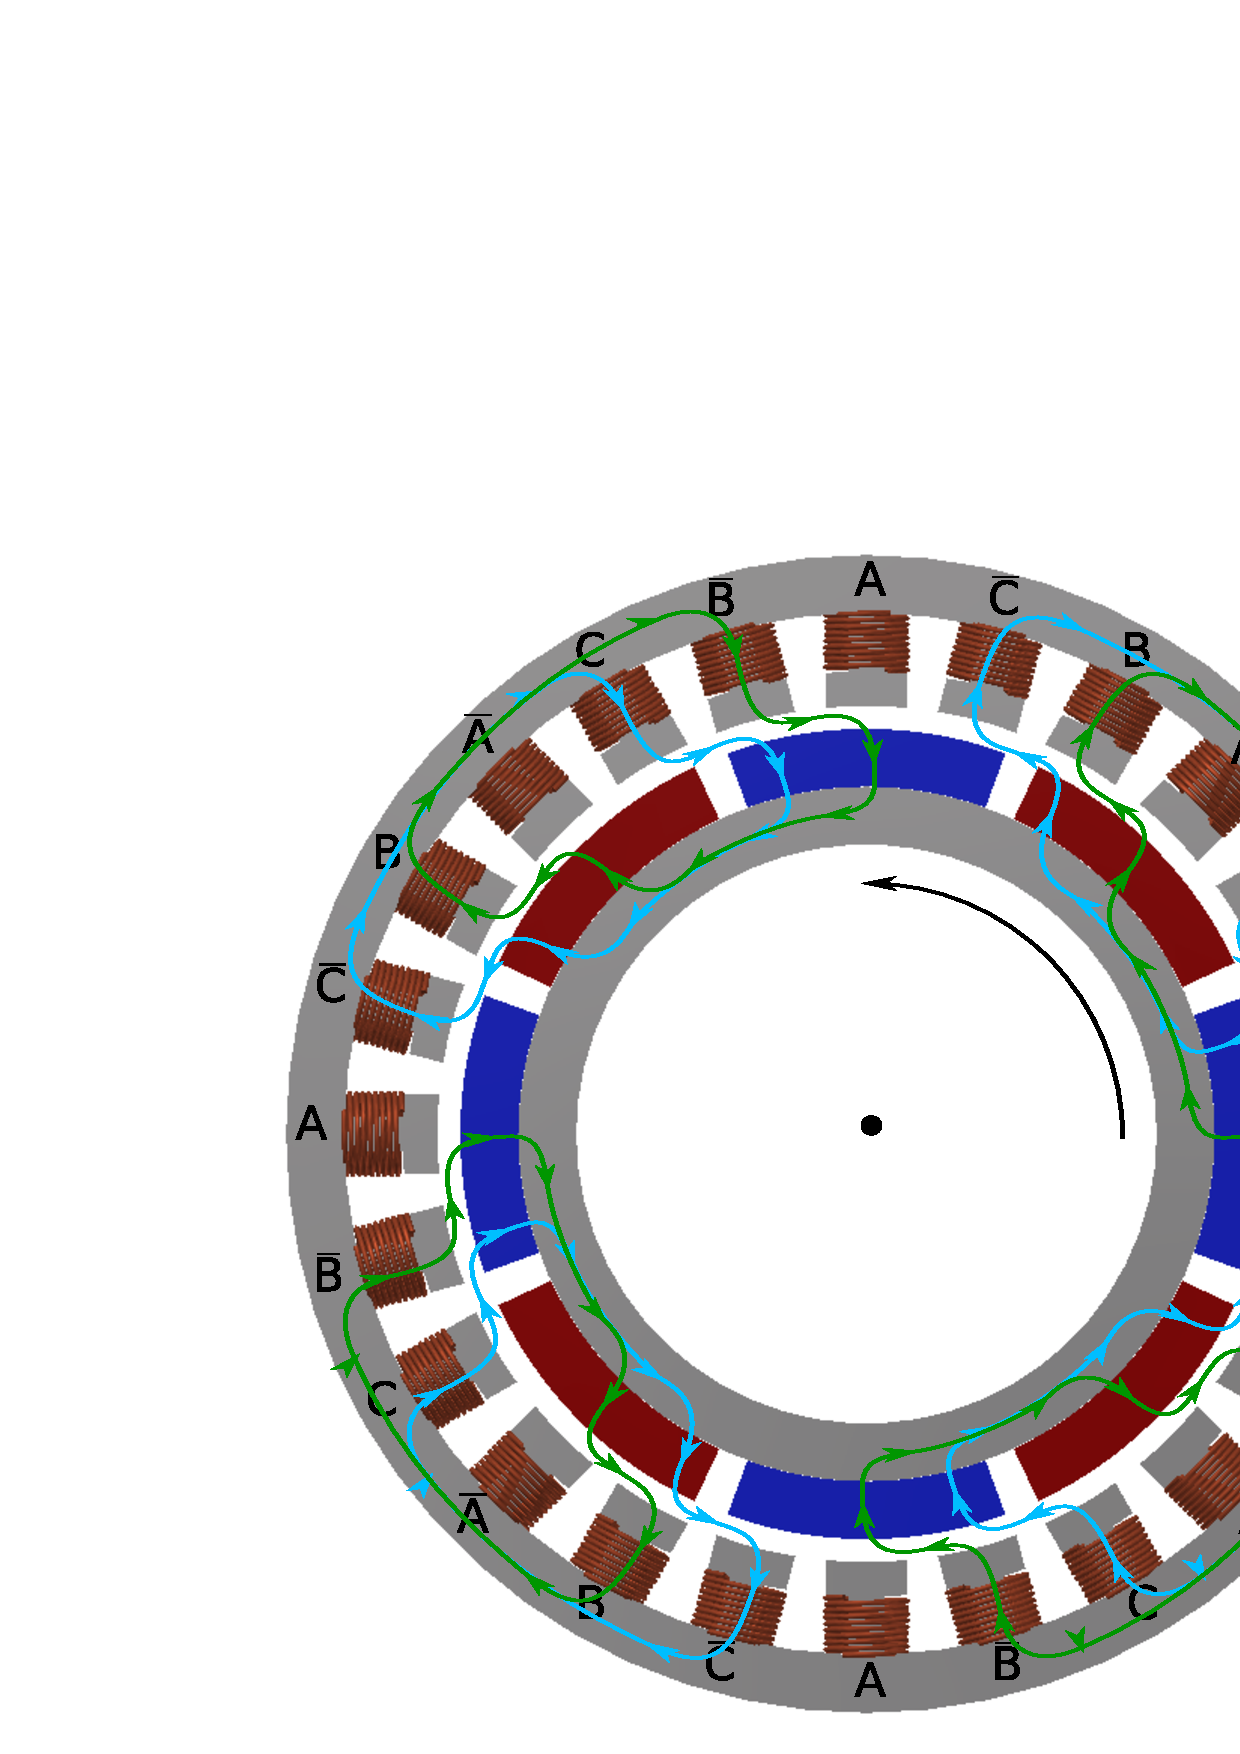
\includegraphics[width=.75\linewidth]{graphics/motor_24p_sketch}
		\caption[Cross section diagram of the motor.]{Cross section diagram of the motor. Magnetic flux lines are drawn in green and cyan for a stator field being 90 electrical degrees ahead of the rotor.}
		\label{fig:motor_24p}
	\end{center}
\end{figure}

According to the manufacturer, the motor is rated for 48VDC and up to 300A for a minute. This corresponds well with its 19hp rating, which means, this DC voltage is the input voltage when driving it as a brushless DC motor, and thus a DC supply voltage of 52.8V does not overload the motor.
However, due to limitations on the power rail the power peaks at 14.7hp.
This happens when equation~\ref{eq:max_power_velocity} is true.
\begin{equation}
V_{BEMF} = \frac{V_{bat}}{2} - I_{max} \cdot R_a
\label{eq:max_power_velocity}
\end{equation}
Using $K_E$ as defined in equation~\ref{eq:KE_definition} to convert the back EMF voltage into a velocity, the maximum power is reached at 3186rpm.
For controlling the motor it can be considered a 2-pole motor, which means that there are only two magnetic fields; the rotor magnetic field generated by the permanent magnets, and the stator field generated by the solenoids. 
This is achieved by converting the measured mechanical angle of the rotor to electrical angle, and then doing all calculations in this domain.

\begin{figure}[H]
	\begin{center}
		\includegraphics[width = .35\linewidth]{graphics/motor_6p}
		\caption{Simplified motor model showing the stator field as green arrows}
		\label{fig:motor_6p}
	\end{center}
\end{figure}

The electric angle of figures~\ref{fig:motor_24p} and~\ref{fig:motor_6p} are the same, and the stator field is set 90 degrees ahead. 
In figure~\ref{fig:motor_6p}, the rotor magnet will always try to line up with the magnetic field lines. 
In the real motor, this will cause the magnetic path to become shorter, as the rotor lines up the permanent magnet poles with the opposite pole of the solenoids. 
By constantly placing the stator field ahead of the rotor, the motor will start moving.
Thus it is necessary to know the position of the rotor in order to determine the angle of the stator field.
For that measurement, an encoder will be used.

\subsection{Definition of Back-EMF Constant and Torque Constant}
The parameters $K_E$ and $K_T$ must be the same for a PMAC motor, since they are dependent on the flux produced in the permanent magnet of the rotor. 
Another reason, that they are the same is, that the motor converts electrical energy to mechanical energy, and electrical energy is the product of current and voltage, and (rotational) mechanical energy is the product of torque and angular velocity. 
A mismatch between $K_E$ and $K_T$ implies, that power appears or disappears, which cannot happen. 

The Back-EMF constant, $K_E$, is defined as the amplitude of each phase-voltage divided with the mechanical angular velocity.

\begin{eqnarray}
K_E =& \frac{V_{BEMF}}{\omega _m}\\
K_T =& \frac{T}{1.5\cdot I_q}
\label{eq:KE_definition}
\end{eqnarray}
This means that $K_E$ and $K_T$ are the same, and the torque produced is the q-current multiplied by $K_T$ and 1.5.
The mathematical reasoning behind is explained by power conservation in equations~\ref{eq:power_electrical_mechanical} through~\ref{eq:mechanical_power_from_electrical}, and by torque contribution in equations~\ref{eq:torque_contributions} through~\ref{eq:torque_function_90deg}. \\

Consider an ideal motor producing some torque, T, and running at a constant angular velocity, $\omega$. 
Losses in the armature resistance and friction are zero. 
The motor is driven by a quadrature current, $I_q$, and a quadrature voltage, $V_q$. 
Currents and voltages along the d-axis are 0. 
The electrical power going into the machine must be equal to the mechanical power going out:

\begin{equation}
P_m = P_e
\label{eq:power_electrical_mechanical}
\end{equation}

Mechanical power is the product of torque and angular velocity:

\begin{equation}
P_m = \omega T
\label{eq:power_mechanical}
\end{equation}

Since there is no phase difference between voltages and currents, electrical power is the product of the RMS values of the current and voltage per phase, times 3:

\begin{equation}
P_e = 3\Big(\frac{1}{\sqrt{2}}V \cdot \frac{1}{\sqrt{2}}I \Big) = V \cdot \frac{3}{2} I
\label{eq:power_electrical_RMS}
\end{equation}

The angular velocity and torque can be calculated from the voltage and current, respectively, and put into equation \ref{eq:power_mechanical}:

\begin{equation}
P_m = \Big( \frac{V}{K_E} \Big) \cdot \big( \frac{3}{2} I \cdot K_T \big)
\label{eq:mechanical_power_from_electrical}
\end{equation}

By setting $K_E = K_T$, equations~\ref{eq:power_electrical_RMS}~and~\ref{eq:mechanical_power_from_electrical} yield the same. \\

Hence, a factor of 1.5 is multiplied to $V\cdot I$ to get the mechanical power. This factor is tied to $K_T$: \\
Consider a motor with with an optimal controller, so the d-current is zero, and the q-current is I. 
The phase current is then calculated by:

\begin{equation}
\begin{bmatrix}
I_a \\ I_b \\ I_c
\end{bmatrix}
=
\begin{bmatrix}
I \cdot \cos(\theta _f) \\ I \cdot \cos(\theta_f - \gamma) \\ I \cdot \cos(\theta_f + \gamma)
\end{bmatrix}
\label{eq:current_q}
\end{equation}

where $\theta_f$ is the electrical angle of magnetic field generated by the stator, and $\gamma = \tfrac{2 \pi}{3}$. In this case, the motor is at constant speed, so the amplitude of all currents are the same.\\
Each of the three phases then contribute to the total torque, depending on the angle between the rotor and the phase, calculated by:

\begin{equation}
\begin{bmatrix}
T_a \\ T_b \\ T_c
\end{bmatrix}
=
\begin{bmatrix}
-I_a \cdot K_T \cdot \sin(\theta _r) \\ -I_b \cdot K_T \cdot \sin(\theta_r - \gamma) \\ -I_c \cdot K_T \cdot \sin(\theta_r + \gamma)
\end{bmatrix}
\label{eq:torque_contributions}
\end{equation}

where $\theta_r$ is the electrical angle of the rotor. \\

The total torque is then the sum of the torque contribution of each phase: 

\begin{equation}
T = T_a + T_b + T_c
\label{eq:total_torque_contribution}
\end{equation}

The torque produced as a function of the angle difference can be calculated with equation~\ref{eq:torque_fucntion_angle}:

\begin{equation}
T(d\theta) = \frac{3}{2} I \cdot K_T \cdot sin(d\theta)
\label{eq:torque_fucntion_angle}
\end{equation}

This can be verified by inspection of figure \ref{fig:torque_contribution_dphi}.
The rotor angle is fixed at 45\si{\degree}. 
$\theta_f$ will go from -135 degrees to 225 degrees. 
Figure~\ref{fig:torque_contribution_dphi} shows torque contribution from each of the three phases, where I and $K_T$ are 1.

\begin{figure}[H]
	\centering
	\includegraphics[width = 10cm]{graphics/torque_contribution_dphi}
	\caption{Torque contribution of each phase as a function of the phase difference}
	\label{fig:torque_contribution_dphi}
\end{figure}
	
	Adding these three contributions gives equation~\ref{eq:torque_fucntion_angle}.
	
	If $d\theta = 90 \si{\degree}$, equation~\ref{eq:torque_fucntion_angle} becomes:
	
\begin{equation}
	T = \frac{3}{2}K_t \cdot I
	\label{eq:torque_function_90deg}
\end{equation}
	
It is easier to measure $K_E$ than $K_T$ and they are defined as the same. \\

\subsection{Motor Parameterization}\label{sub:1117_param}
Due to the sparse information available from the manufacturer of the motor, it is necessary to measure some of the parameters of the motor. 
It will also be necessary to determine exactly what these parameters define, since the manufacturer has not defined certain things such as what current measurement is related to torque through $K_T$.
Parameters to determine are the back-EMF constant, $K_E$, the armature resistance, $R_a$, and the armature inductance, $L_a$.
Each of the following sections describe the procedure used to find each of these parameters. 

\subsubsection{Measuring Back-EMF Constant}\label{sub:KE-KT}
To find $K_E$, a hand-held power drill is used to rotate the motor at a constant speed. 
An oscilloscope with a differential probe is used to measure the voltage between two of the phases. 
Because of the high input impedance of the differential probe, there is no current and thus the armature inductance and resistance can be neglected. 
The peak-peak voltage and the corresponding frequency is noted in the table below:

\begin{table}[!h]
\begin{center}
\begin{tabular}{S|S}
	{Frequency }[\si{\hertz}]  & {Voltage } [\si{\volt}$_{\text{pp}}$] \\
	\hline
	23.49 & 9.7  \\
	38.32 & 15.3\\
	40.97 & 16.5\\
	44.9 & 17.7\\
	54.7 & 21.8\\
	61.81 & 24.2\\
	72.13 & 28.3
\end{tabular}
\end{center}
\caption{Measured line-line voltage at electrical frequencies}
\label{tab:KE_measurements}
\end{table}

The phase amplitude of the voltage is calculated by dividing the voltages in table~\ref*{tab:KE_measurements} with $2\sqrt{3}$. The mechanical angular velocity is calculated by multiplying the frequency in table~\ref*{tab:KE_measurements} with $2\pi$, and dividing with $4$ pole pairs. 
The resultant voltages and velocities are divided to calculate $K_E$, and the average is calculated for these. 
The result is:

\begin{equation}\label{eq:K_E}
K_E = K_T = 0.0733 \si{\volt\second\per\radian}
\end{equation}

with a spread of 1.3\%. 
According to the datasheet, $K_T$ is 0.13. 
This is 1.77 times higher than the measured $K_E$. 
There are two potential reasons for this.
One is, that the manufacturer uses line-to-line currents and voltages instead, since the difference is close to $\sqrt{3}$. 
Another possible reason is, that the manufacturer defines $K_T$ as the torque produced with the given q-current, in which case $K_T = 1.5K_E$, and the measured $K_T$ is about 15\% below the manufacturer's datasheet. 
Whatever the reason, equation~\ref{eq:K_E} will be used throughout this report. \\

This means, the maximum speed and torque can be calculated:

\begin{equation}
\omega _{max} = \frac{V_{bat}}{2 K_E} = 360 \si{\radian \per \s} 
\label{eq:max_rotational_speed}
\end{equation}

\begin{equation}
T_{max} = I_{max} \cdot \frac{3}{2} K_T = 33 Nm
\label{eq:max_torque}
\end{equation}

\subsubsection{Armature Resistance}\label{sub:R_a-measurements}
To measure the armature resistance, a high DC current is driven through one terminal to the other. 
The voltage at the terminal is measured.
The large current causes a significant voltage drop in the wires leading from the power supply to the motor. 
Based on the measured voltages and currents the resistance between the two terminals can be calculated.
The results are shown in the table below:

\begin{table}[h]
	\begin{center}
	\begin{tabular}{r | c | c | c}
		{Terminals} 	& {V} [\si{\volt}]	& {I} [\si{\ampere}]	& {R} [\si{\milli\ohm}] \\
		\hline
		{AB} 			& 0.217 		& 17.93 		& 12.10  \\
		\hline
		{AC}			& 0.206  		& 17.96 		& 11.47  \\
		\hline
		{BC}			& 0.235 		& 17.93  		& 13.11
	\end{tabular}
	\end{center}
	\caption{Measured DC resistance across terminal-pairs.}
	\label{tab:armature_resistance}
\end{table}

It is desirable to know the resistance from one terminal to the common star point. 
That can be calculated by equation~\ref{eq:resistance_converter}

\begin{equation}
R_a = \frac{R_{AB} + R_{AC} - R_{BC}}{2}
\label{eq:resistance_converter}
\end{equation}

This gives different armature resistances for different phases ranging from 5.2 to 6.9 \si{\milli\ohm}. 
This is about half the line-to-line resistance listed by the manufacturer at 13\si{\milli\ohm}. 
However, since the motor is a wye connection, knowing the resistance between a terminal and the star-point is more helpful when modeling the motor.

\subsubsection{Armature Inductance}\label{sub:L_A-measurements}
In order to measure the winding inductance of the motor, a full bridge driver is used to generate a square wave at different frequencies. 
The two terminals of the full bridge driver is connected to terminals B and C, and voltage and current is measured.
The motor is not moving, so there is no back-EMF. 
The resistor voltage is subtracted from the voltage measurements, and what remains is the inductor voltage. 
Current and voltage has been plotted in figure~\ref{fig:20kHz_squarewave}.  

\begin{figure}[H]
	\begin{center}
		\includegraphics[width = 10cm]{graphics/inductance_measured_v_i}
		\caption{20 kHz square wave voltage and the resulting current.}
		\label{fig:20kHz_squarewave}
	\end{center}
\end{figure}

These waveforms have been measured at 5 kHz, 10 kHz, 20 kHz and 30 kHz. 
For this project a switching frequency of 20 kHz will be used, so only this plots will be shown. 
Due to the high sampling rate of the oscilloscope and low bit resolution, differentiating the current will yield very large spikes for short periods of time. 
Therefore, the current, time and voltage measurements will be periodically averaged and downsampled by a factor of 70. 
The derivative of the current is then calculated by:

\begin{equation}
\frac{di}{dt}[n] = \frac{i[n]-i[n-1]}{t[n]-t[n-1]}
\end{equation}

This is the derivative of the current at the point immediately between two samples, so to synchronize the time and voltage arrays, each two consecutive samples are averaged. 
The resulting waveforms are plotted in figure~\ref{fig:20kHz_squarewave_di}

\begin{figure}[h]
	\begin{center}
		\includegraphics[width = 12cm]{graphics/20kHz_v_di}
		\caption{20 kHz square wave voltage and derivative of the resulting current.}
		\label{fig:20kHz_squarewave_di}
	\end{center}
\end{figure}

It appears, that there is some proportionality between the derivative of the current, and the voltage across this inductor.

The inductance is generally lower than the terminal-to-terminal inductance provided by the manufacturer of 0.1 \si{\milli\henry}. 
The average inductance varies a bit with different frequencies, and 20 kHz is actually the lowest.

\begin{table}[H]
	\begin{center}
	\begin{tabular}{S | S | S}
		{Frequency} [\si{\kilo\hertz}] 	& 	{Average inductance} [\si{\milli\henry}] & 	{Current ripple} [\si{\ampere}] \\
		\hline
		5			&	0.946					&	16.83 \\
		\hline
		10	    	&	0.844					&	12.10 \\
		\hline
		20			&	0.632					&	7.13 \\
		\hline
		30 			&	0.879					&	5.25 
	\end{tabular}
	\caption{Average of measured inductance and current ripple at different frequencies.}
	\label{tab:inductance_and_current_ripple}
	\end{center}
\end{table}

The inductances in table~\ref{tab:inductance_and_current_ripple} is the inductance from one terminal to another, so the per-phase inductance will be half.
The inductance determines the phase shift on the sinusoidal voltages and currents driving the motor, and the current ripple at the switching frequency.
The maximum frequency of these are determined by the maximum rotational speed of the motor calculated in equation~\ref{eq:max_rotational_speed}, which equals 229 \si{\hertz}.
So when modelling the motor, one must settle on a value of $L_d$ and $L_q$ that is close to the the low frequency inductance of 0.473 \si{\milli\henry}, and the higher frequency inductance of 0.316 \si{\milli\henry}. 
For modelling the motor, an inductance of 0.4 \si{\milli\henry} will be used for both $L_d$ and $L_q$. 

\subsection{Parking Test}\label{sub:parking_test}
The encoder is positioned on the axle of the motor at an unknown angle. 
Since this will not change, a one time parking test will be performed, where current will be passed into one terminal and out of the other two. 
This will be done with a DC power supply with current limit. 
The motor should position itself at one of four mechanical angles spaced 90\si{\degree} apart. 
This offset will be subtracted from any angular readings.\\

The motor is parked with 30\si{\ampere}. 
The test is repeated to determine all four parking spots for each phase, and the angles are shown in table~\ref{tab:parking_angles}. 
The phases A, B and C correspond to the terminals with the names M1, M2 and M3 etched into the case of motor. 

\begin{table}[H]
	\centering
	\sisetup{table-space-text-post=\si{\degree}}
	\begin{tabular}{|S | S | S | S|}
		\hline
		{Quadrant} & {Phase A } & {Phase B } & {Phase C } \\
		\hline
		{First} & {43.6\si{\degree}} & {75.9\si{\degree}} & {16.9\si{\degree}} \\
		\hline
		{Second} & {132.2\si{\degree}} & {167.3\si{\degree}} & {101.3\si{\degree}} \\
		\hline
		{Third} & {223.6\si{\degree}} & {257.3\si{\degree}} & {194.1\si{\degree}} \\
		\hline
		{Fourth} & {312.2\si{\degree}} & {348.8\si{\degree}} & {279.8\si{\degree}} \\
		\hline
	\end{tabular}
	\caption{Parking angles for the encoder.}
	\label{tab:parking_angles}
\end{table}

The four parking angles of each phase should be spaced 90 degrees from each other. 
The parking angles in one quadrant should be spaced 30 degrees apart.
This does not hold true for all values - both columns A and B are spaced 90\si{\degree} apart within the precision of the encoder, but the difference between phase A and B in the same quadrant are spaced 34.45\si{\degree} apart.
Column C varies from 84\si{\degree} to 97\si{\degree}, however they are on average spaced 30\si{\degree} from Column A. 
This should definitely not be the case, but  the reason is currently unknown. 
For the controller, the Phase A readings will be used throughout the report. 
The angles are then wrapped down to the first quadrant by subtracting 90, 180 and 270 degrees from second, third and fourth quadrant respectively, and the average is calculated to be 42.9\si{\degree}, corresponding to a value of 30.5\si{\degree} from the encoder. 
Whenever the rotor position is read, 30.5 will be subtracted from the value. 

It should also be noted, that the order of the phases is A, B and C, which is the opposite order of the one described in section~\ref{sub:motor_descrpition}. 
This means, that the encoder counts down when the go-kart is moving forward. 
\newpage
\section{Motor Modelling}
To model the PMSM motor an equivalent circuit of the motor will be used. Figure \ref{fig:PMSM_Equivalent} shows this circuit.

\begin{figure}[H]
	\centering
	\includegraphics[width=.95\linewidth]{graphics/PMSM_Equivalent}
	\caption{PMSM motor equivalent circuit, source:  }
	\label{fig:PMSM_Equivalent}
\end{figure}

\todo{Morten: find better picture of this, or make it. source of this pic: MORTEN}

\subsection{State Space Model}
A state space model is derived from the physical representation of a PMSM motor, figure \ref{fig:State_space_model1}, consisting of an electrical part on the left and a mechanical part on the right side of the model. The model is made in MatLab Simulink. The model is very similar to that of a DC motor when interpreted like this.

\begin{figure}[H]
	\centering
	\includegraphics[width=.95\linewidth]{graphics/State_space_model1}
	\caption{PMSM motor state space model.}
	\label{fig:State_space_model1}
\end{figure}

Reducing this model to use transfer functions for the electrical and mechanical parts results in a more simple model, figure \ref{fig:State_space_model2}. A wind resistance has been added to show how it affects the torque of the motor. The value of the wind resistance is the rotational speed squared multiplied by a drag value. This value will be a negative number, which is then added to the torque output to slow down the motor. The drag can be approximated by looking at the gearings of the kart and the motors own drag coefficient.

\begin{figure}[H]
	\centering
	\includegraphics[width=.95\linewidth]{graphics/State_space_model2}
	\caption{PMSM motor model simplified with tranfer functions.}
	\label{fig:State_space_model2}
\end{figure}

An even further reduced model is derived to further simplify the system. This model removes torque load, friction and wind resistance. It is shows on figure \ref{fig:State_space_model3}. This model can be used to find controller values if the torque load, viscous friction and wind resistance are all seen as disturbances. The controller should be able to handle the about of disturbance that can be found in these values.

\begin{figure}[H]
	\centering
	\includegraphics[width=.95\linewidth]{graphics/State_space_model3}
	\caption{PMSM motor model without torque load, friction and wind resistance.}
	\label{fig:State_space_model3}
\end{figure}

\subsection{Controlling Current}
The motor must be current controlled in order to limit the torque. If the motor was speed controlled, as is often used in motor control, it could demand a much higher current than possible by the circuit, requiring a limiter on the current input instead, or otherwise it could result in destroying the drive circuit. A current control also means that the speeder pedal will be a current reference, translating into a torque reference, resulting in an even motor speed even if the kart is driving on a uneven plane such as a hill.

A control loop is added to the model, figure \ref{fig:State_space_model4}. It must be current controlled to control the torque. This means that a feedback loop is added from inside the motor back to the controller. 

\begin{figure}[H]
	\centering
	\includegraphics[width=.95\linewidth]{graphics/State_space_model4}
	\caption{PMSM motor model with a current control loop.}
	\label{fig:State_space_model4}
\end{figure}


\subsection{Transfer Function}
The model of figure \ref{fig:State_space_model4} can be rearranged to simplify the transfer function. This rearrangement can be seen on figure \ref{fig:State_space_model5}. Here the current is the output, a current reference is the input, and the mechanical part of the motor is all placed into a feedback loop.

\begin{figure}[H]
	\centering
	\includegraphics[width=.95\linewidth]{graphics/State_space_model5}
	\caption{PMSM motor model rearranged to simplify the transfer function.}
	\label{fig:State_space_model5}
\end{figure}

\begin{figure}[H]
	\centering
	\includegraphics[width=.95\linewidth]{graphics/State_space_model6}
	\caption{PMSM motor model as a plant with PI control}
	\label{fig:State_space_model6}
\end{figure}

Using masons rule \todo{Morten: dodds book reference to masons} the transfer function can be derived. Seeing the control loop as a controller and a plant the following equation is achieved. Equation \ref{eq:plant_masons}.

\begin{equation}
\frac{I_m}{I_{ref}}= \frac{(K_p+K_i\frac{1}{s})G(s)}{1-(K_p+K_i \frac{1}{s})G(s)}
\label{eq:plant_masons}
\end{equation}

Replacing $G(s)$ and rearranging to get the form of a characteristics equation the transfer function is equation \ref{eq:transfer_function_full}.
\begin{equation}
\frac{I_m}{I_{ref}}=\frac{s^2\frac{K_p}{L}+s(\frac{K_i}{L}+\frac{K_pK_v}{J})+\frac{K_iK_v}{J_r}}{s^3+s^2(\frac{R}{2L}+\frac{K_v}{J}+\frac{K_p}{L})+s(\frac{3K_t^2}{2JL}+\frac{K_vR}{JL}+\frac{K_i}{L}+\frac{K_pK_v}{2J})+\frac{K_iK_v}{J}}
\label{eq:transfer_function_full}
\end{equation}

This third order transfer function will be used to derive the controller values.

\subsection{Controller Values}
To find the controller values the Stephen Dodds Settling Time Formula for $5\%$ settling time is used. The desired characteristics polynomial of a transfer function for the settling time formula to work is

\begin{equation}
s^n+d_{n-1}s^{n-1}+\cdot \cdot \cdot +d_1s+d_0
\end{equation}

The d's of a given order can be looked up in Stephen J. Dodds' book \todo{cite book} on page 850.

This yields the following third order equation for a third order system.

\begin{equation}
s^3 + 3\alpha s^2+3\alpha^2s+\alpha^3
\end{equation}

Based on the transfer function in equation ref and a settling time of 0.1 seconds, alpha will be defined by the following equation. This value is used to find the Kp and Ki values for the controller.

\begin{equation}
\alpha=\frac{1.5(1+n)}{T_s^{5\%}}=\frac{6}{0.1}=60
\label{eq:Dodds_settlingtime}
\end{equation}

Finding the controller values.

\begin{equation}
3 \alpha= \frac{R}{2L}+ \frac{K_v}{J}+ \frac{K_p}{L} \rightarrow K_p=(3 \alpha - \frac{K_v}{J}- \frac{R}{2L})L
\end{equation}
\begin{equation}
3 \alpha^2= \frac{2K_t^2}{2JL}+ \frac{K_vR}{JL}+ \frac{K_i}{L}+ \frac{K_pK_v}{2J} \rightarrow K_i=(3 \alpha^2- \frac{K_pK_v}{2J}- \frac{K_vR}{JL}- \frac{3K_t^2}{2JL})L
\end{equation}

These equations yield the following controller values, equation \ref{eq:Kpvalue} and \ref{eq:Kivalue}.
\begin{equation}
K_p=0.0039
\label{eq:Kpvalue}
\end{equation}
\begin{equation}
K_i=0.4606
\label{eq:Kivalue}
\end{equation}

\subsection{Simulation}
Testing the $K_p$ and $K_i$ values should result in a stable current output from the electrical part of the motor, which is desired to control the torque. This simulation will add the $K_p$ and $K_i$ values to the control loop and review the outcome.



\clearpage
\section{Simulation}\label{sec:Simulations}

Simulation tools have been a great help, not only understanding the electromechanical system, and design a controller from it, but estimating requirements for the electric components. Primarily, Simscape has been used, but Plecs has also been used specifically to simulate the inverter. This section will explain how the model has been build, starting with the mechanical system, then the motor model, the transformation and control part, and finally the three-phase switching pole. 

\subsection{Mechanical System}\label{sub:Simulations_mec}
The mechanical system consists of a mass of the gokart with driver, turbulent air resistance, wheels and a gear. While there are a lot of interesting blocks in the Simscape $\rightarrow$ SimDriveline library, we will stick with the mechanical library, because this is detailed enough, and more easy to port to Plecs. 

\begin{figure}[H]
	\includegraphics[width=15cm]{graphics/simulations_mechanical_full.png}
	\caption{Block diagram of the mechanical system}
	\label{fig:mechanical_full}
\end{figure}

Figure~\ref{fig:mechanical_full} shows the block diagram of the mechanical part, that the motor will drive. Starting from the left, the Permanent Magnet Synchronous Motor is the motor and the Ideal Rotational Motion Sensor is used for the Clarke-Park transformations. The first inertia block contains both the inertia of the motor, which is 0.0052, and the motor-side gear. It is possible to add inertias that are connected to the same mechanical rod. The inertia of the gear depends on its size. Assuming, that the gear is a disc, the mass is calculated by equation~\ref{eq:mass of disc}:

\begin{equation}
m_{G1} = \rho \pi r^2 \cdot h
\label{eq:mass of disc}
\end{equation}

where rho is the mass density of iron of $7870 \dfrac{kg}{m^3}$, r is the radius, and h is the thickness of 7 mm. Radius is defined by the number of teeth, G1, of the gear and the pitch, which is the distance between two adjacent teeth, which is 12.5 mm. Hence the radius can be calculated by equation. Inertia of a disc depends on mass and radius of the disc.

\begin{equation}
	r=\frac{G \cdot pitch}{2 \pi}
	\label{eq:radius_from_G}
\end{equation}

\begin{equation}
J_G = \frac{mr^2}{2} = \frac{\rho \pi r^2 \cdot h \cdot r^2}{2} = G^4 \frac{\rho \pi \frac{pitch}{2 \pi} \cdot h}{2} \approx 1.36 \cdot 10^{-9} G^4
\label{eq:inertia_of_disc}
\end{equation}

This equation is used to dertermine the inertia of the two cogs, the motor-side cog, G1, has 12 teeth, and the wheel-side cog, G2, has 50 teeth. This ratio, G2/G1 is put into the block "Wheel and Axle".

The mass is set to 200 -- 250 kg, depending on the driver, and this includes the mass of the car. This is a high estimate. A lower value could make the controller less stable, but a higher value will heat up the inverter more. 

Turbulent friction caused by the wind resistance is calculated by equation~\ref{eq:wind_resistance}.

\begin{equation}
F=-\frac{1}{2} \rho A c v^2
\label{eq:win_resistance}
\end{equation}

where $\rho$ is the density of air, A is the frontal area, c is the drag coefficient and v is the speed. The frontal area has been approximated to two boxes with the combined area of $0.6 m^2$\todo{add a picture of a go kart with two boxes across it, the lower one being 1 m wide, and 0.4 m high, and the second one being 0.5 m wide an 0.4 m high. mba}. The density of air is approximately $1.225 \frac{kg}{m^3}$, and the constant c is approximately 0.8, according to a paper about air resistance found online. The constants are multiplied into one constant called c\_drag, as shown in equation~\ref{eq:cdrag}
%"http://www.torvergata-karting.it/filemanager/download/191/The%20evaluation%20of%20aerodynamic%20drag%20of%20go-karts%20by%20means%20of%20coast%20down%20test%20and%20CFD%20analysis.pdf"
These constants are put into the gain block, "Drag coefficient", and multiplied by the square of the speed. The result is put into an ideal force source. 

\begin{equation}
F=-c_{drag} v^2 = -0.296 v^2
\label{eq:cdrag}
\end{equation}

This system can be simplified, so that all inertia an mass become one block and the gear and wheel can be removed. This is done by a set of rules that apply for this mechanical circuit: The gear box reduces the speed, and increases torque. Torque is force times radius, and speed is angular velocity times radius.
To turn the mass, m, into a inertia, assume a cylindrical shell with radius r, and mass m. Inertia is then calculated by:

\begin{equation}
J=mr^2
\end{equation}

This inertia can then be added to the inertia J\_G2. Same rules apply for a gear as for a transformer when reflecting a load from one side to the other, as shown in equation~\ref{eq:inertia_reflect}

\begin{equation}
J_{ref} = \frac{G1^2}{G2^2} J
\label{eq:inertia_reflect}
\end{equation}

This inertia is then added to the inertia of the motor and J\_G1:

\begin{equation}
J = (mr^2+J_{G2}) \cdot \big(\tfrac{G1}{G2}\big)^2 + J_{G1}+J_M
\end{equation}

For a mass of 250 kg, this comes to $0.282 kg m^2$.

In equation~\ref{eq:win_resistance}, speed can be replaced with angular velocity and a gain, and force can be replaced by torque and a gain. So the equation becomes this:

\begin{equation}
\frac{T G2}{r G1} = c_{drag} \big(\omega r \tfrac{G1}{G2}\big)^2
\end{equation}

isolating T, and putting $\omega$ by it self, we get:

\begin{equation}
T= c_{drag} \Big(\frac{G1 r}{G2}\Big)^3 \omega^2 \approx -11.1\cdot 10^{-6} \omega^2
\end{equation}

The mechanical diagram is reduced to figure ~\ref{fig:reduced_mechanical_system}

\begin{figure}[H]
	\begin{center}
	\includegraphics[width=12cm]{graphics/simulations_mechanical_simplified.png}
	\caption{Block diagram of the reduced mechanical system}
	\label{fig:reduce_mechanical_system}
	\end{center}
\end{figure}

His can be ported to Plecs, where all the used mechanical parts exist. Only difference is, that the inertia block is placed inline with the wire, and not as an appendage.

\subsection{Motor Model}\label{sub:motor_model_simscape}
The Permanent Magnet Synchronous Motor is found in Simscape $\rightarrow$ SimPowerSystem $\rightarrow$ Simscape Components $\rightarrow$ Machines $\rightarrow$ Permanent Magnet Rotor. This is a quite simple model, with only four parameters: Number of pole pairs, flux linkage of the magnet, inductance and armature resistance. The parameters can be seen on figure~\ref{fig:pmsm_parameters_simscape}. A similar block can be found in Plecs under Electrical $\rightarrow$ Machines. This model has the same parameters as in Simscape, but also inertia and friction.

\begin{figure}[H]
	\centering
	\begin{subfigure}[t]{.49\linewidth}
		\centering
		\includegraphics[width=\textwidth]{graphics/PMSM_simulink.png}
		\label{fig:pmsm_parameters_simscape}
		\caption{Simscape PMSM parameters.}
	\end{subfigure}
	\begin{subfigure}[t]{.39\linewidth}
		\centering
		\includegraphics[width=\textwidth]{graphics/PMSM_Plecs.png}
		\label{fig:pmsm_parameters_Plecs}
		\caption{Plecs PMSM parameters.}
	\end{subfigure}
	\label{fig:pmsm_parameters_plecs_simscape}
	\caption{Comparison of Simscape and Plecs models of the Permanent Magnet Synchronous Motor.}
\end{figure} 

One thing to note in both cases is, that the flux linkage is divided by the number of pole pairs. The reason for this is likely a matter of definitions, and the relation has been deduced using simulations. Armature resistance and inductances are per-phase, and the values used are found in section~\ref{sub:1117_param}.

\subsection{Electrical Network and control}\label{sub:sim_electrical}
This is where, the Simulink and Plecs block diagram differ a lot. The purpose of using Simulink is that it's quick and easy to change multiple parameters in order to develop and test a controller. The advantage in Plecs its ability to simulate switchmode power electronics, where there's a vast ratio between the minimum timestep defined by the switching frequencies, and the duration of the simulation. The sparse electrical network along with the discrete controller and modulation blocks have been shown in figure~\ref{fig:simulations_electrical}.

\begin{figure}[h]
	\begin{center}
	\includegraphics[width=16cm]{graphics/simulations_electrical.png}
	\caption{Block diagram of the Simulink electrical network and modulation.}
	\label{fig:simulations_electrical}
	\end{center}
\end{figure}

The motor block has an external connection to neutral, which the real motor doesn't have. This neutral seems to need a dc path to ground, and so does the controlled voltage sources. Since the external ground cannot be connected to the internal star point of the motor, the connection is made with a very large resistor of $1 G\Omega$. The lighter blue wire going into the "\~" port of the PMSM block is a three phase electrical cable, which is used throughout the SimPowerSystem sublibrary, and the Splitter collects three wires into a cable. \\

Current is sensed on wires A and B, and used to calculate $I_C$ in the upper part of the block diagram. The signal goes to a Clarke-Park transformation block outside figure~\ref{fig:simulations_electrical}, and returns as $I_d$ and $I_q$ on the bottom left part of the picture. \\

The angular position is measured with an ideal position sensor, and then sent to the encoder block. Here, the finite precision of the encoder is simulated by the equation~\ref{eq:Encoder_block_function}

\begin{equation}
output = floor \Bigg(\frac{\phi \cdot 256}{2 \pi} \% 256 \Bigg)
\label{eq:Encoder_block_function}
\end{equation}

where \% is the mod function. The purpose of that is to wrap the output to a value between 0 and 255, which can be used for look-up tables. The floor function rounds a number, effectively quantizing the output. It has been attempted to use the quantizer block, but that causes stiffness to the point where the simulations almost stall. The output is sent to the Zybo block, which will be explained in section~\ref{sub:sim_zybo}.\\

The Zybo generates duty cycles for each phase ranging from -1 to 1. This value is then multiplied with half the DC voltage, and saturated, o the ideal voltage sources do not provide more voltage than the battery can.

\subsubsection{Plecs model}\label{sub:sim_plecs_electrical}
As said, the Plecs model differs vastly from the Simulink model in the electrical network, as it more closely resemble the real analog circuit. It is presented on figure~\ref{fig:plecs_electrical}.

\begin{figure}[H]
	\begin{center}
		\includegraphics[width = \textwidth]{graphics/Plecs_electrical.pdf}
		\label{fig:plecs_electrical}
		\caption{Block diagram for the svm plecs simlations.}
	\end{center}
\end{figure}

\subsection{Zybo block}\label{sub:sim_zybo}
%!TEX root = ../main.tex
\section{System Implementation and Testing}
This section will describe how the system was implemented and tested on both a test setup and the real go-kart setup. 

\subsection{Test Setup}
In order to test subparts of the complete system a test setup was introduced.
It consists of a permanent magnet motor of the type PM5113 with a RMB28MD encoder module mounted with a small distance to the end of the shaft.
The setup furthermore consits of a 74HCT14 level shift interface board and a ?? dual H-bridge and can be seen in figure \ref{fig:small_motor_setup}.
The setup was made and soldered by the supervisors of the project.
The full setup with H-bridge can be used to test the functionality of the Embedded System.
The motor and encoder can be used to test the full system.

\begin{figure}[!h]
	\centering
	\includegraphics[width=0.8\linewidth]{graphics/small_motor_setup}
	\caption[Test setup.]{Test setup with PM5113 motor.}
	\label{fig:small_motor_setup}
\end{figure}

\todo[inline]{The figure is wrong!! signal should go two times in the level shifter - Mikkel}

\subsection{Test of Embedded System}

\section{Conclusion}
Throughout this report has been described the various steps taken to create a control system for an electric go-kart.
As part of this, circuit boards were developed to take care of over current protection, scaling of signals and various other tasks.
The OCP was simulated in order to verify its functionality
However, except for the driver board, due to time constraints it was not possible to finish the boards in time for the deadline.
A driver board was made to for the DRV8301, the driver chip used in the project.
This board was made to work with a test setup which includes the inverter developed, a small PMAC motor and some temporary boards made to interface the signals of the system.
Using this test setup it was possible to drive the motor, verifying that the inverter is functional.
A controller for the system was created using the settling time formulae.
The controller was tested using the extensive simulations made of the system using Simulink.
The controller was discretized in preparation for using it on the embedded system.
This was unfortunately not tested.
The embedded system was programmed using khaOS, a Run To Complete Scheduler.
Its real time performance was verified using an oscilloscope.\\

Many parts of the project were not completed to the satisfaction of the group.
Throughout there were problems with delivery of components as well as the quality of the boards created.
This resulted in much time spent doing things not necessarily conducive to a better end product.

\newpage
\begin{thebibliography}{11} %This number should be higher than the number of entries in the bibliography because reasons...
%	\bibitem{id}
%		Author(s) Last name, First name, Company/Organisation, Year. Full Title
	\bibitem{feedback}
			Dodds, Stephen J., University of East London, 2015. Feedback Control: Linear, Nonlinear and Robust Techniques and Design with Industrial Applications.
	\bibitem{z7010}
			Xilinx, Nov. 2015. Zynq-7000 All Programmable SoC (Z-7010, Z-7015 and Z-7020): DC and AC Switching Characteristics.
	\bibitem{bootstrap_paper}
			Fairchild, Dec. 2014, Design and Application Guide of Bootstrap Circuit for High-Voltage Gate-Driver IC.
	\bibitem{DRV8301}
			Texas Instruments, Aug. 2013, DRV8301 - Three Phase Pre-Driver with Dual Current Shunt Amplifiers and Buck Regulator (datasheet).
	\bibitem{IRF4468PbF}
			International Rectifier, IRFP4468PbF Power MOSFET datasheet
	\bibitem{power_switching_converters}
			Neacsu, Dorin O., 2016, Power-Switching Converters: Medium and High Power-Switching 
	\bibitem{adc}
		Xilinx, May. 2015, 7 Series FPGAs and Zynq-7000 All Programmable SoC XADC Dual 12-Bit 1 MSPS Analog-to-Digital Converter (User Guide).	
	\bibitem{superB}
		Super B Lithium batteries, SB12V20P-FC Lightweight Lithium ion starter battery datasheet
	\bibitem{zynq_reference}
		Xilinx, February. 2015, Zynq-7000 All Programmable SoC (Technical Reference Manual).
	\bibitem{third_harmonic_injection}
		Suda, Barath Kumar; David, James, Eaton Corporation, Mar 'A Novel Third Harmonic Injection Method for Closed Loop Control of PMSM Motors'
	\bibitem{pmac_equivalent_diagram}
		A. B. Dehkordi, Student Member, IEEE, A. M. Gole, Senior Member, IEEE, T. L. Maguire, Senior Member, IEEE; 'Permanent Magnet Synchronous Machine Model for
		Real- Time Simulation'
	\bibitem{TO_247}
		Vishay Siliconix, July. 2013, TO-247AC (High Voltage) Package Information
	\bibitem{gokart_constant}
		Biancolini, Marco Evangelos, Department of Mechanical Engineering Tor Vergata University, 'Evaluation Of Aerodynamic Drag Of Go Kart By Means Of Coast Down Test And Cfd Analysis'
	\bibitem{wire_inductance}
		Thomsen, Mark, 1999, IEEE, 'Tricks of the Trade: Guesstimating Inductance of Wire Loops'
	\bibitem{electric_motor_and_drives}
		Austin Hughes, Bill Drury; 'Electric Motors and Drives: Fundamentals, Types and Applications - Fourth Edition'


\end{thebibliography}
\newpage
\appendix
%\section{Board Layout}
\label{app:boardlayout}

\end{document}

